% !TeX program = pdfLaTeX
\documentclass[smallextended]{svjour3}       % onecolumn (second format)
%\documentclass[twocolumn]{svjour3}          % twocolumn
%
\smartqed  % flush right qed marks, e.g. at end of proof
%
\usepackage{amsmath}
\usepackage{graphicx}
\usepackage[utf8]{inputenc}

\usepackage[hyphens]{url} % not crucial - just used below for the URL
\usepackage{hyperref}
\providecommand{\tightlist}{%
  \setlength{\itemsep}{0pt}\setlength{\parskip}{0pt}}

%
% \usepackage{mathptmx}      % use Times fonts if available on your TeX system
%
% insert here the call for the packages your document requires
%\usepackage{latexsym}
% etc.
%
% please place your own definitions here and don't use \def but
% \newcommand{}{}
%
% Insert the name of "your journal" with
% \journalname{myjournal}
%

%% load any required packages here



% Pandoc citation processing

\usepackage{xcolor}
\usepackage{booktabs}
\usepackage{longtable}
\usepackage{array}
\usepackage{multirow}
\usepackage{wrapfig}
\usepackage{float}
\usepackage{colortbl}
\usepackage{pdflscape}
\usepackage{tabu}
\usepackage{threeparttable}
\usepackage{threeparttablex}
\usepackage[normalem]{ulem}
\usepackage{makecell}
\usepackage{xcolor}

\begin{document}

\title{Correlates of Cycling Flows in Hamilton, Ontario - Fastest, Quietest, or
Balanced Routes? }



\author{  Elise Desjardins \and  Christopher D. Higgins \and  Darren M. Scott \and  Emma Apatu \and  Antonio Páez \and  }


\institute{
        Elise Desjardins \at
     School of Geography and Earth Sciences, McMaster University \\
     \email{\href{mailto:desjae@mcmaster.ca}{\nolinkurl{desjae@mcmaster.ca}}}  %  \\
%             \emph{Present address:} of F. Author  %  if needed
    \and
        Christopher D. Higgins \at
     Department of Human Geography, University of Toronto \\
     \email{\href{mailto:cd.higgins@utoronto.ca}{\nolinkurl{cd.higgins@utoronto.ca}}}  %  \\
%             \emph{Present address:} of F. Author  %  if needed
    \and
        Darren M. Scott \at
     School of Geography and Earth Sciences, McMaster University \\
     \email{\href{mailto:scottdm@mcmaster.ca}{\nolinkurl{scottdm@mcmaster.ca}}}  %  \\
%             \emph{Present address:} of F. Author  %  if needed
    \and
        Emma Apatu \at
     Department of Health Research Methods, Evidence, and Impact, McMaster
 University \\
     \email{\href{mailto:apatue@mcmaster.ca}{\nolinkurl{apatue@mcmaster.ca}}}  %  \\
%             \emph{Present address:} of F. Author  %  if needed
    \and
        Antonio Páez \at
     School of Geography and Earth Sciences, McMaster University \\
     \email{\href{mailto:paezha@mcmaster.ca}{\nolinkurl{paezha@mcmaster.ca}}}  %  \\
%             \emph{Present address:} of F. Author  %  if needed
    \and
    }

\date{Received: date / Accepted: date}
% The correct dates will be entered by the editor


\maketitle

\begin{abstract}
Cycling is an increasingly popular mode of travel in Canadian urban
areas, like the Greater Toronto and Hamilton Area (GTHA). While trip
origins and destinations can be inferred from travel surveys, data on
route choice is often not collected which makes it challenging to
capture the attributes of routes travelled by cyclists. With new
algorithms for cycle routing it is now possible to infer routes. Using
bicycle trip records from the most recent regional travel survey, a
spatial interaction model is developed to investigate the built
environment correlates of cycling flows in Hamilton, Ontario, a
mid-sized city part of the GTHA. A feature of the analysis is the use of
CycleStreets to compare the distance and time according to different
routes inferred between trip zones of origin and destination. In
addition, network autocorrelation is accounted for in the estimated
models. The most parsimonious model suggests that shortest-path quietest
routes that minimize traffic best explain the pattern of bicycle trip
flows in Hamilton. Commercial and office locations and points of
interest at the zone of origin negatively correlate with the production
of trips, while different land uses and the availability of jobs at the
zone of destination are trip attractors. The use of a route planner
offers a novel approach to modelling and understanding cycling flows
within a city. This may be useful for transportation planners to infer
different types of routes that cyclists may seek out and consider these
in travel demand models.
\\
\keywords{
        cycling \and
        spatial interaction modelling \and
        route choice \and
    }


\end{abstract}


\def\spacingset#1{\renewcommand{\baselinestretch}%
{#1}\small\normalsize} \spacingset{1}


\hypertarget{sec:intro}{%
\section{Introduction}\label{sec:intro}}

Cycling is an increasingly popular mode of travel in Canadian urban
areas. From 1996 to 2016 the number of people commuting to work by
bicycle in Canadian census metropolitan areas increased by 87.9\% and
the share of bicycle commute trips grew from 1.2\% to 1.6\% (Statistics
Canada 2017). Such modal shifts have been prompted in part by the widely
recognized health and environmental benefits associated with cycling.
Compared to other transportation modes, travelling by bicycle is more
enjoyable (Páez and Whalen 2010), and is associated with better
self-perceived health (Avila-Palencia et al. 2018) and reduced risk of
chronic disease (Celis-Morales, Lyall, and Welsh 2017; Oja et al. 2011).
Furthermore, cycling also leads to reduced greenhouse gas emissions
(Zahabi et al. 2016) and improved air and noise pollution (De Nazelle et
al. 2011). These benefits serve as motivation for cities to encourage
more travel by this mode, but this requires effort to put cycling on par
with other modes of transportation at a policy level. For this reason,
many Canadian cities have integrated cycling in their transportation
plans in recent years (\emph{inter alia}, see City of Calgary 2011; City
of Montreal 2017; City of Vancouver 2012) and have implemented a range
of interventions and strategies that have been effective in increasing
cycling (Assunçao-Denis and Tomalty 2019; Verlinden, Y and Manaugh, K
and Savan, B and Smith Lea, N and Tomalty, R and Winters, M 2019).

The City of Hamilton, a mid-sized city located in the Greater Toronto
and Hamilton Area (GTHA) urban region approximately 50 km from Toronto,
has experienced an increase in cycling. Approximately one third of all
trips in this area are 5 km or less, which is widely considered to be a
bikeable distance. In 2016, 1.2\% of all trips in Hamilton were made by
bicycle according to the latest \emph{Transportation Tomorrow Survey},
the regional travel survey conducted every 5 years (Data Management
Group 2018). This was a two-fold increase from the 2011 survey results
when the cycling mode share was only 0.6\% (Data Management Group 2014).
Hamilton has also been identified as a city where cycling levels could
substantially increase to approximately 35\% of the mode share (Mitra et
al. 2016). The increase in bicycle trips in Hamilton between 2011 and
2016 occurred over the same period that cycling interventions were
implemented, such as new cycling facilities and a public bicycle-share
program. In other words, we suggest that Hamilton can be characterized
as a developing cycling city (see Liu et al. 2020) because efforts to
increase cycling have been implemented and cycling levels are growing.
Recent studies in Hamilton have used global positioning system (GPS)
data from the bike share program to conduct route choice analysis (Lu,
Scott, and Dalumpines 2018; Scott, Lu, and Brown 2021) and explore
influences on bike share ridership (Scott and Ciuro 2019). However, we
still know relatively little about trips in this city beyond those made
by bike share. To date, there has been no published research that has
investigated the pattern of bicycle trips in Hamilton using data from
the 2016 \emph{Transportation Tomorrow Survey}. Our understanding of the
spatial distribution of such trips in a mid-sized developing cycling
city and the influence of the built environment is also limited.

To address these gaps in knowledge, the objective of this study is to
investigate the correlates of cycling flows in Hamilton. This paper
describes the development of a spatial interaction model (a component of
the four-step travel model; see Dios Ortúzar and Willumsen 2011) to test
the level of cycling flows against various attributes at the zones of
origin and destination. Travel surveys are typically rich in terms of
information about where trips start or end, but are less informative
with respect to route characteristics, which often have to be inferred.
For this reason, a feature of the analysis is the use of an algorithm
for cycle routing, \emph{CycleStreets}, to infer and compare different
routes between the zones of origin and destination instead of using only
the shortest-path distance. This algorithm identifies routes according
to various attributes and characterizes them as \emph{fastest},
\emph{quietest}, and \emph{balanced} routes. The distance and time from
the zone of origin to destination along each inferred route serve as
measures of cost in the analysis. The following two questions are
addressed: 1) \emph{Which attributes at the zones of origin and
destination influence cycling trip flows in Hamilton?}; and 2)
\emph{Which type of route best explains the pattern of cycling trip
flows in Hamilton?} In addition, residuals from the spatial interaction
model are analyzed using a spatial autocorrelation statistic to assess
the model's compliance with the assumption of independently distributed
residuals. Future opportunities for research and practice, including
assessment of the built environment along select routes identified by
the algorithm, are also discussed.

Following recommendations for reproducible research in the spatial
sciences (see Brunsdon and Comber 2020), all data and code used in this
paper are available online. The source for this paper is an R markdown
document that can be obtained from the following GitHub repository:

\begin{quote}
\url{https://github.com/paezha/Correlates-of-Cycling-Flows-Route-Types}
\end{quote}

\hypertarget{sec:background}{%
\section{Background}\label{sec:background}}

A diversity of factors influence the decision to commute by bicycle
ranging from the natural and built environments to individual and
household characteristics (Heinen, van Wee, and Maat 2010). Where people
live, work, and play is particularly important because it influences the
transport modes available to them, the destinations and amenities that
they can access, and the routes they can travel to get from A to B. As
such, the built environment receives a lot of attention in cycling
research because factors that are known to influence cycling can be
modified by urban and transportation planners to potentially shift a
large number of currently motorized trips. Population-based travel
surveys are useful for understanding cycling activity and patterns at
the city level (Handy, van Wee, and Kroesen 2014) which can, in turn,
support strategic investments where cycling levels have the potential to
increase. Open source tools, such R packages and OpenStreetMap, can also
assist in geographic analysis at the local level to complement and
inform transport planning decisions and practice (Lovelace 2021).

The \emph{behavioral model of the environment} was proposed as a
theoretical framework for environmental audits to identify the
determinants of walking and cycling at three different scales that make
up any trip (Moudon and Lee 2003). According to this framework, all
three spatial areas (i.e., the characteristics of i) the origin, ii) the
destination, and iii) the route) are important and necessary to assess
the influence of the built environment on walking and cycling. These
modes, more so than motorized travel, allow a traveller to interact more
intimately with the micro-level environment (Moniruzzaman and Páez 2012,
2016; Moudon and Lee 2003). This type of framework holds true for
bicycle trip analysis as well. Winters et al.~(2010) conducted a study
measuring built environment variables at three different scales in
Vancouver, Canada and found that the built environment around the origin
and destination, as well as along the route, are indeed different and
influence cycling in different ways. This emphasizes the need for travel
behaviour models to capture environmental attributes along different
parts of the trip, not just at the zone of origin and destination or the
community-level.

\hypertarget{macro}{%
\subsection{Macro-Level Built Environment Factors}\label{macro}}

The urban form at the places where bicycle trips originate and end is
important (Scott and Ciuro 2019). This topic is well-documented in the
cycling literature. Land use mix, whereby people can reach a variety of
amenities within a distance that is comfortable to cycle, influences
travel by bicycle (Cervero, Denman, and Jin 2019; Sallis et al. 2013;
Winters et al. 2010; Zhao 2014). For instance, Heesch et al.~(2015)
found that shorter distances to destinations, including a business
district with jobs and a river where there are bicycle paths, increased
the odds of cycling in Brisbane, Australia. Higher densities of
population (Nielsen and Skov-Petersen 2018; Nordengen et al. 2019;
Schneider and Stefanich 2015; Winters et al. 2010) and employment (Le,
Buehler, and Hankey 2018; Zhao 2014) are other important factors. In the
case of cities with low levels of cycling, access to bicycles can make
this mode more attractive. Cole-Hunter et al.~(2015) report that public
bicycle share stations near the residence were a significant positive
determinant of commuting by bicycle. The quality of the urban
environment also matters. Areas with trees and green space also
associated with more cycling (Cole-Hunter et al. 2015; Le, Buehler, and
Hankey 2018; Mertens et al. 2017).

In most studies, a combination of these attributes are found to
influence cycling, which suggests that multiple factors are needed to
create spaces that ultimately encourage people to cycle (Cervero,
Denman, and Jin 2019; Handy 2020). Higher levels of cycling are
typically observed in neighbourhoods with good street connectivity,
supportive infrastructure, and a variety of amenities that can be
reached in a short distance. However, there is variation in the relative
influence of these attributes across studies and across places, which
might reveal different effects that are related to contextual
behaviours, or planning and transportation policies. For example,
residential density (Scott and Ciuro 2019; Zhao 2014) and the presence
of cycling infrastructure (Moudon et al. 2005) are not always a
significant factor. Therefore, additional analysis to determine the
influence of specific attributes on cycling levels is important in
developing cycling cities, where such studies have not been previously
conducted, which can inform new strategies to induce the uptake of
cycling.

\hypertarget{route}{%
\subsection{Micro-Level Route Factors}\label{route}}

Cycling infrastructure is often identified as an important attribute in
bicycle-friendly cities. It is thought to be fundamental for encouraging
more bicycle trips in cities that are predominantly car-centric (Adam,
Jones, and te Brömmelstroet 2020). The provision of, or proximity to,
infrastructure has been found to have a influence or association with
cycling behaviour (\emph{inter alia}, see Buehler and Pucher 2012;
Buehler and Dill 2016; Dill and Carr 2003; Mertens et al. 2017; Winters
et al. 2010). For example, Le et al.~(2018) found that cycling
facilities had a strong association with bicycle volume and traffic
based on their analysis of 20 metropolitan statistical areas in the
United States. Infrastructure can be very influential - a new bicycle
lane in Oslo, Norway attracted trips by shifting cyclists from other
parallel routes (Pritchard, Bucher, and Frøyen 2019). Cyclists also
detour from dominant routes to incorporate cycling facilities in their
travels (Scott, Lu, and Brown 2021). This suggests that it is not
uncommon for preferred routes to change as new facilities are built over
time and they are incorporated into daily trips. Furthermore,
infrastructure can also increase perceptions of cycling safety
(Branion-Calles et al. 2019) which may encourage more trips. At the very
least, cycling infrastructure is a visual and physical sign that streets
can accommodate people who choose to travel using this mode.

Studies examining the characteristics along routes travelled by people
who cycle is limited but has grown over the past decade owing in part to
the availability of new data technologies. Researchers have used a
variety of methods to reveal the preferences of cyclists including data
obtained from global positioning system (GPS) devices or smartphone
applications (Pritchard 2018). In general, studies using such data
confirm that people who cycle prefer routes with separated facilities
over mixing with traffic (Chen, Shen, and Childress 2018; Dill 2009;
El-Assi, Mahmoud, and Habib 2017; Lu, Scott, and Dalumpines 2018;
Skov-Petersen et al. 2018) and incorporate infrastructure as part of
their routes (Dill 2009; Lu, Scott, and Dalumpines 2018; Pritchard,
Bucher, and Frøyen 2019; Scott, Lu, and Brown 2021). One study conducted
in Portland, Oregon using GPS data found that streets with bike lanes
were comparable in attractiveness to streets with low traffic volume
(Broach, Dill, and Gliebe 2012). By examining GPS data from Hamilton's
bike share program, Lu et al.~(2018) found that users travel routes that
are significantly longer than the shortest path distance and are more
likely to use local streets with low traffic and bicycle facilities.
Similarly, Chen et al.~(2018) also reported that people who travel by
bicycle in Seattle, Washington prefer short and flat routes with
connected facilities on roads that have low traffic speeds. Their study
found more variability with respect to preference for views along routes
with features like mixed land use, street trees, lighting, and city
features.

Cycling facilities and street connectivity have most consistently been
found to be an important attribute of the built environment for
promoting cycling (Yang et al. 2019). However, few studies incorporate
variables at two or more spatial scales, as outlined in Moudon and Lee's
(2003) framework to capture a comprehensive view of the variability in
the built environment that a cyclist might encounter. Winters et al.'s
(2010) study in Vancouver, Canada is an exception, as is a recent study
conducted by Cole-Hunter et al.~(2015) that took some factors at the
route level into account in their analysis of cycling propensity in
Barcelona, Spain. Nielsen and Skov-Petersen (2018) recently analyzed the
influence of built environment attributes at three different scales on
the probability of cycling in Copenhagen, Denmark which captured some of
the spatial differentiation at which variables are important, however
they did not include any route analysis. There is a need for more
research to measure and understand the built environment attributes that
affect cycling along different parts of the trip and at different
spatial zones.

\hypertarget{sec:method}{%
\section{Methods}\label{sec:method}}

\hypertarget{model}{%
\subsection{Spatial Interaction Modelling}\label{model}}

We use spatial interaction methods to analyze bicycle trip flows in
Hamilton, Ontario. In the form of a gravity model, this modelling
approach can account for multiple spatial zones along a cycling trip,
and is therefore a more holistic approach than trip generation analysis
(e.g.~Dios Ortúzar and Willumsen 2011, chap. 5). The
\emph{Transportation Tomorrow Survey} provides sufficient information to
infer the zone of origin and destination of all bicycle trips in
Hamilton using centroids of the traffic zones. Built environment
attributes at the zone of origin and zone of destination of cycling
trips can be accessed through publicly available data. Finally, new
algorithms for cycle routing like \emph{CycleStreets} now make it
possible to infer route characteristics between origins and
destinations, which can be considered when calculating the cost (i.e.,
in terms of distance and time) of undertaking trips.

Spatial interaction models operate on principles of propulsion,
attraction, and the friction of space (Rodrigue 2020). We can assume
that there are factors within a particular geographic area that
contribute to producing or generating trips, such as residential or
population density, and there are factors in other geographic areas that
attract trips like jobs or amenities. Finally, there is the friction of
space, in other words, the cost incurred in reaching a destination from
an origin. Spatial interaction models are useful for estimating or
explaining variation of spatial flows in a particular system or to
predict them in different scenarios.

The spatial interaction model is generally represented by the following
expression: \begin{equation}
\label{eq:interaction-model}
U_{ij} = f(V_i, Wj, d_{ij})
\end{equation}

\noindent where \(i\) represents the origin, \(j\) represents the
destination, \(U_{ij}\) is the total interaction between origin and
destination (i.e., for this analysis it is the number of bicycle trips
recorded in the \emph{TTS}), \(V_i\) is a vector of attributes at the
zone of origin (i.e., the push factors), \(W_j\) is a vector of
attributes at the zone of destination (i.e., the pull factors), and
\(d_{ij}\) represents the cost of making the trip (i.e., often the
distance or time as a measurement of spatial separation).

Poisson regression is commonly used in the estimation of a spatial
interaction model when the dependent variable is available as a count
(Chun 2008; Griffith 2011; Metulini, Patuelli, and Griffith 2018). This
specification of the gravity model estimates the level of flows based on
explanatory variables at the origin and destination (Griffith and
Fischer 2016). This regression model is also suitable for datasets that
contain true zero counts (Griffith 2011), as is the case when many zones
of origin and destination do not generate trips. The Poisson model is:
\begin{equation}
\label{eq:poisson-model}
P(U_{ij}|x,\theta) = \frac{\lambda^U_{ij}}{U_{ij}!}e^{-\lambda} 
\end{equation}

To estimate the model, we work with the mean function \(\lambda\):
\begin{equation}
\label{eq:mean-function}
\lambda = e^{\theta^\prime x} 
\end{equation}

The generalized linear version of the model uses the natural logarithm
as the link function, which leads to the following log-linear
specification of the mean function (see Chun 2008): \begin{equation}
\label{eq:link-function}
ln(U_{ij}) = \theta_0 + \theta_O ln(V_i) + \theta_Dln(W_j) + \theta_C ln(d_{ij}) 
\end{equation}

In Equation \ref{eq:link-function}, \(x = [1, V_i, W_j, d_{ij}]\) is the
vector of correlates including constant term(s), variables at the origin
(\(V_i\)), at the destination (\(W_j\)), and the cost of movement
between origin and destination (\(d_{ij}\)). These correlates are
associated with a vector of estimable parameters
\(\theta = [\theta_0, \theta_O, \theta_D, \theta_C]\) corresponding to
the constant term(s), and the variables at the origin, at the
destination, and the cost.

For our analysis, bicycle trip counts serve as the dependent variable
and built environment or demographic attributes known to influence
cycling serve as independent variables, with \(V_i\) and \(W_j\)
representing push and pull factors at \(i\) and \(j\) respectively, and
\(d_{ij}\) the cost or separation between the zone of origin \(i\) and
zone of destination \(j\).

As highlighted by numerous studies (e.g., Chun 2008; Metulini, Patuelli,
and Griffith 2018), spatial or network autocorrelation can occur in
spatial interaction models because of, among other things, unobservable
factors at the zone of origin or destination that are not included in
the model, or a misspecified cost function. Failing to account for
network autocorrelation can lead to unreliable findings or misleading
interpretations of the behaviour modelled (Chun 2008; Griffith and
Fischer 2016). In this respect, use of Moran's \(I\) has been criticized
for the case of residuals of a Poisson regression model because it is
based on a normality assumption and Poisson has distributional
properties that are not well known (Chun 2008). Instead the \(T\)
statistic (see Jacqmin-Gadda et al. 1997) is recommended for
applications in spatial interaction modelling (Chun 2008; Metulini,
Patuelli, and Griffith 2018).

The \(T\) statistic derived by Jacqmin-Gadda et al.~(1997) has the
following equation: \begin{equation}
\label{eq:T-statistic}
T = \sum_{i=1}^{N} \sum_{j\ne{i}}^{N} w_{ij}(Y_i - \hat{\mu_i})(Y_j - \hat{\mu_j})
\end{equation}

In Equation \ref{eq:T-statistic}, the term \(w_{ij}\) is a weight that
indicates whether, and if so to what extent, zones \(i\) and \(j\) are
related in space (conventionally \(0\le w_{ij}\le 1\)); \(Y_i\) is a
spatial random variable, and \(\hat{\mu_i}\) is the estimated value of
the variable according to a suitable model.

\hypertarget{study-area}{%
\subsection{Study Area}\label{study-area}}

Hamilton is a growing mid-sized city located in the Greater Toronto and
Hamilton Area, in Canada. The city is divided by the Niagara Escarpment,
which separates the lower city and downtown core in Dundas Valley from
the suburban/rural parts of the city on top of the escarpment and is
approximately 100m tall in many places. The population was approximately
540,000 in 2016 at the time that the \emph{Transportation Tomorrow
Survey} was conducted, but is expected to increase by 22.9\% over the
coming 15 years (City of Hamilton 2018a), indicating that transportation
demand will likely also grow. The city's current Cycling Master Plan was
released in 2009 to ``guide the development and operation of {[}the
city's{]} cycling infrastructure for the next twenty years'' (City of
Hamilton 2018c, i) and was most recently updated in 2018 (City of
Hamilton 2018b). According to the City of Hamilton, approximately 46\%
of the planned city-wide cycling infrastructure, which includes
on-street and off-street facilities, has been built as of 2019. Around
15 to 20 km of new cycling facilities are built each year, amounting to
an annual increase of 1-2\% for the entire network.

\begin{figure}
\centering
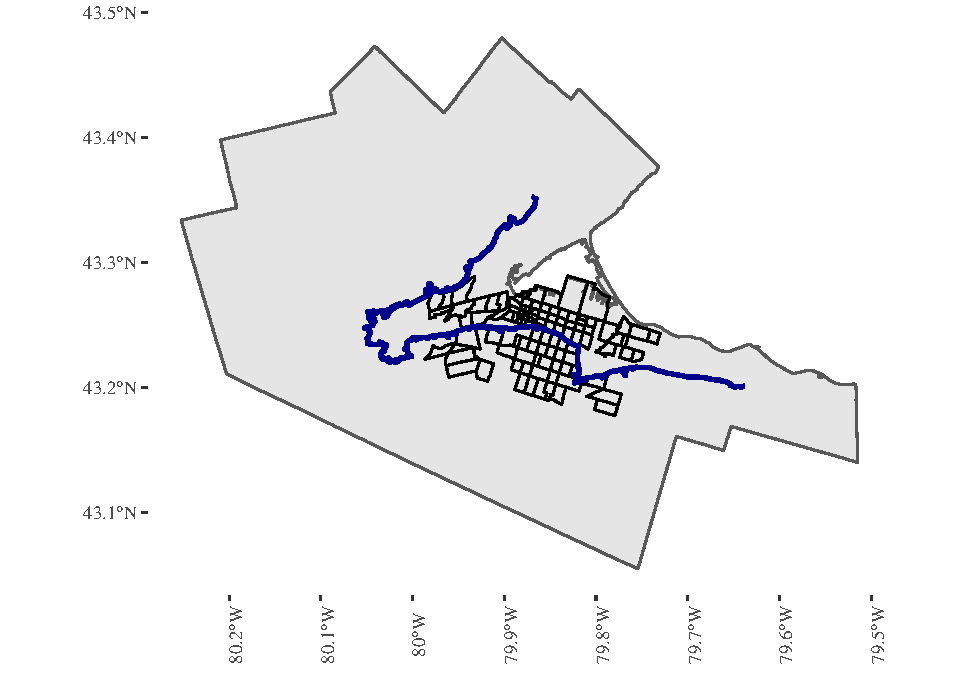
\includegraphics{Correlates-cycling-flows-routes_files/figure-latex/context-plot-1.pdf}
\caption{\label{fig:context-plot} Traffic analysis zones in Hamilton's
census metropolitan area that generated at least one bicycle trip are
outlined in black. The Niagara Escarpment, which can be as high as 100
metres in many places, is outlined in dark blue.}
\end{figure}

\begin{figure}
\centering
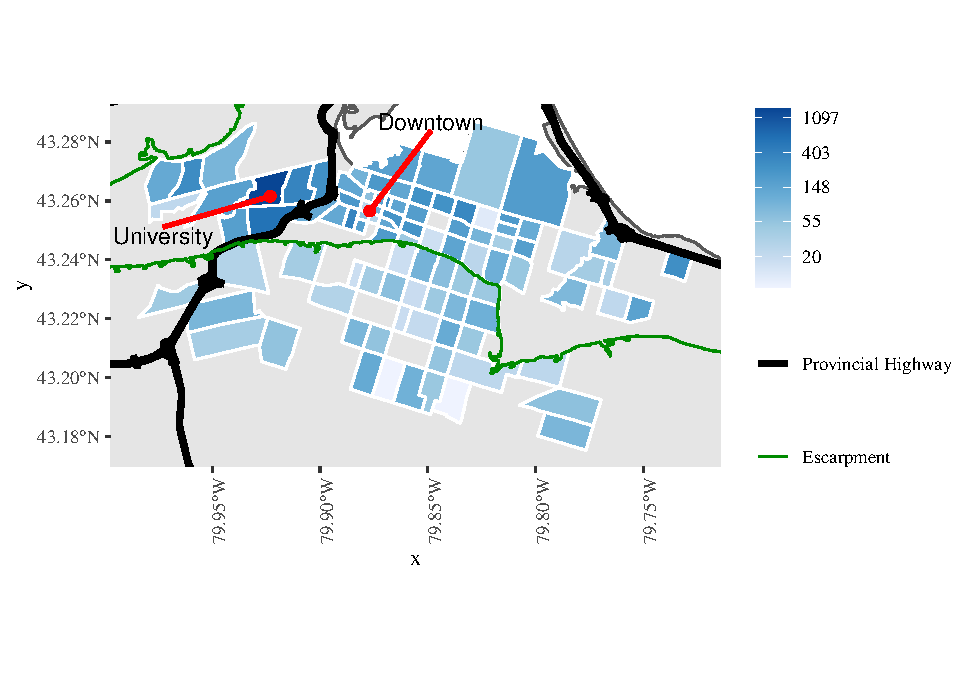
\includegraphics{Correlates-cycling-flows-routes_files/figure-latex/trips-by-origin-1.pdf}
\caption{\label{fig:trips-by-origin} Number of Trips Produced by Each
Traffic Zone (Black lines are provincial highways and green line is the
Niagara Escarpment)}
\end{figure}

\hypertarget{data-sources}{%
\subsection{Data Sources}\label{data-sources}}

The \emph{Transportation Tomorrow Survey} (\emph{TTS}) is a voluntary
travel survey conducted every 5 years since 1986 to collect information
about urban travel for commuting purposes in Southern Ontario (Data
Management Group 2018). The final dataset for the 2016 survey includes
6,424 completed surveys in Hamilton out of a total of 162,708 from the
entire GTHA. The results from respondents in Hamilton serve as the
primary dataset used in this analysis and were made available in Spring
2018. The \emph{TTS} study employed a mixed sampling approach that was
primarily address-based in response to changes in landline ownership and
increasing households that only have a cell phone and no landline (Data
Management Group 2018). The survey includes sampling weights to obtain
population-level values of the variables (Data Management Group 2018).
The survey was conducted between September and December 2016 online
(64\% of surveys completed) and by telephone (36\% of surveys
completed). Each participant was asked to provide household and
demographic data (e.g., household size, number of vehicles, gender,
etc.) and to describe all trips (e.g., origin, destination, transport
mode, etc.) made the previous day by each member of the household aged
11 years or older. Trip data are aggregated for public use and the
\emph{traffic zone} is the finest level of spatial disaggregation.
Hamilton has 234 traffic zones. Each traffic zone typically falls along
the centre line of roads or the natural geographic boundaries, but may
or may not align with municipal ward boundaries.

In total, there are 13,635 bicycle trips in the 113 traffic zones within
Hamilton, after the expansion factor to make it a representative sample.
The trips occurred between a total of 294 origin-destination pairs. The
true origins and destinations of trips are not included in the dataset,
only the number of trips produced or attracted to each \emph{traffic
zone}. Although cycling increased overall in the city in recent years,
levels vary across different parts of the city. The geographical context
for the analysis can be seen in Figure \ref{fig:context-plot}. The
maximum number of bicycle trips recorded to or from a traffic zone was
365 trips. This traffic zone features the local university. This aligns
with Scott and Ciuro's (2019) findings that the university is a major
generator and attractor of bike share trips. Due to low density and few
destinations within a bikeable distance, the majority of traffic zones
located in the rural areas of the city generated 0 bicycle trips. An
average of 46 bicycle trips occurred per traffic zone that produced
bicycle trips. The minimum number of bicycle trips recorded in a traffic
zone that produced any trips at all was 6. Of the 113 traffic zones that
produced bicycle trips, about 25\% produced more than 55 trips, likely
zones that feature attributes that are conducive to greater cycling
levels, such infrastructure or mixed land uses.

Objectively measured demographic and environmental attributes at the
zones of origin and destination that might explain the production or
attraction of bicycle trips were included in the model. These
explanatory variables were selected based on their known or potential
influence on cycling behaviour, as identified in the literature above,
but also on our ability to access such data. For instance, residential
density at the zone of origin might explain why trips begin there, and
the number of jobs or services at the zone of destination could explain
why trips end there. When possible, the datasets used for this analysis
come from 2016 to match the year of the \emph{Transportation Tomorrow
Survey} results. The \emph{2016 Canadian Census}, which is publicly
available information, provided population estimates at the census tract
level. Land use data was accessed from \emph{Teranet Inc.} and The City
of Hamilton's Department of Planning and Economic Development. The
latter dataset defines all land parcels in the city as well as the type
of land use for each parcel. The 2016 \emph{Enhanced Points of Interest}
(EPOI), produced by DMTI Spatial Inc, is a national database of over 1
million business and recreational points of interest in Canada that
featured over 32,000 points of interest located in Hamilton. Finally,
The City of Hamilton's \emph{Open Data Program} offered a dataset
containing the number of transit stops and the number of existing and
proposed cycling infrastructure segments.

\hypertarget{data-preparation}{%
\subsection{Data Preparation}\label{data-preparation}}

Hamilton's bicycle trip records were accessed in July 2019 and exported
as a contingency table with the traffic zones of origin and destination
of all cycling trips. The original table containing only trip
information featured 294 origin-destination (O-D) pairs of traffic
zones. This table was cleaned to remove 13 isolated zones, which
produced trips only to neighbouring zones and not elsewhere in the city.
This reduced the number of O-D pairs in our analysis from 294 to 262.
Objective demographic and environmental variables were geographically
organized in two different zoning systems, and areal interpolation was
performed to convert census data from the tract level to traffic zones.
Similarly, spatial subsetting was performed to select and organize
environmental attributes based on their known coordinates and whether or
not they intersected with a traffic zone. Zonal demographic and
environmental variables were then joined to the origin-destination
table. Table \ref{tab:variables} shows the variables that were tested in
the model to measure their relative and collective influence on cycling
trip flows.

\begin{table}

\caption{\label{tab:data-sources}\label{tab:variables}Demographic and Built Environment Variables Used in the Analysis}
\centering
\resizebox{\linewidth}{!}{
\fontsize{9}{11}\selectfont
\begin{tabular}[t]{>{}l|>{\raggedright\arraybackslash}p{30em}|>{}l}
\toprule
Variable & Description & Source\\
\midrule
\em{\cellcolor{gray!6}{Population}} & \cellcolor{gray!6}{Persons residing in each traffic zone (1,000s)} & \cellcolor{gray!6}{2016 Canadian Census}\\
\em{Points of Interest} & Points of interest (e.g., health care and educational facilities, restaurants, etc.) per traffic zone  (1,000s) & DMTI Spatial Inc.\\
\em{\cellcolor{gray!6}{Bus Stops}} & \cellcolor{gray!6}{Municipal bus stops per traffic zone  (100s)} & \cellcolor{gray!6}{City of Hamilton Open Data}\\
\em{Infrastructure Segments} & Existing and proposed cycling infrastructure segments (100s) & City of Hamilton Open Data\\
\em{\cellcolor{gray!6}{Institutions}} & \cellcolor{gray!6}{Institutions (e.g., schools, places of worship, government, etc.) per traffic zone  (1,000s)} & \cellcolor{gray!6}{Teranet Inc., Hamilton Parcel/Land Use Data}\\
\addlinespace
\em{Commercial} & Commercial locations (e.g., general retail, recreation, and sports clubs, etc.) per traffic zone (1,000s) & Teranet Inc., Hamilton Parcel/Land Use Data\\
\em{\cellcolor{gray!6}{Residential}} & \cellcolor{gray!6}{Residences (e.g., detached house, semi-detached house, apartment, etc.) per traffic zone (1,000s)} & \cellcolor{gray!6}{Teranet Inc., Hamilton Parcel/Land Use Data}\\
\em{Full-Time Jobs} & Persons employed full-time, outside of the home, by zone of employment (1,000s) & Transportation Tomorrow Survey\\
\em{\cellcolor{gray!6}{Part-Time Jobs}} & \cellcolor{gray!6}{Persons employed part-time, outside of the home, by zone of employment (1,000s)} & \cellcolor{gray!6}{Transportation Tomorrow Survey}\\
\bottomrule
\end{tabular}}
\end{table}

In addition to the variables in Table \ref{tab:variables}, dummy
variables were created to account for Hamilton's topography. Traffic
zones were classified by geographic area, namely zones in the lower city
and zones in the Niagara Escarpment or the suburban/rural parts of the
city. This classification was used to code O-D pairs that were in the
same different geographical classes, to capture that a cyclist would
need to navigate changes in elevation and natural features when
travelling across different topographies in Hamilton. If both the zone
of origin and zone of destination were in the lower city, this pair was
labelled with 0. If the origin and destination were in different regions
(i.e., lower city and escarpment/rural), the pair was labelled with 1.
If both zones were in the escarpment or rural areas, the pair was
labelled with 2.

\hypertarget{inferring-cycle-routes}{%
\subsection{Inferring Cycle Routes}\label{inferring-cycle-routes}}

The \emph{Transportation Tomorrow Survey} does not ask respondents to
state the routes that they travel, so this information is unknown. For
this reason, we have to infer routes using the centroids of each traffic
zone polygon as a start or end point, which are then used as cost
functions in the model. We use a novel routing service,
\emph{CycleStreets}\footnote{https://www.cyclestreets.net/}, to this
end. The algorithm relies on data that is publicly available through
OpenStreetMap, so there are additional objectively measured
environmental variables captured in the cost function. This can
potentially provide more information about trip distribution than using
only the shortest-path distance. The distance and time on each leg of a
route can be obtained from the algorithm, and from these, the total
travel distance and time for each type of route between origin and
destination can be calculated.

The algorithm infers three different types of routes: \emph{fastest},
\emph{quietest}, and \emph{balanced}. The \texttt{R}
package\footnote{https://CRAN.R-project.org/package=cyclestreets} used
in this analysis states: ``These represent routes taken to minimize
time, avoid traffic, and compromise between the two, respectively''
(Lovelace and Lucas-Smith 2018, 1). The documentation states that the
algorithm considers the following factors when searching for a route:
length of streets, signalled junctions, signalled crossings, elevation,
speed, busynance, and quietness. The \emph{CycleStreets} algorithm rates
the \emph{quietness} as a percentage score, with routes featuring cycle
tracks and park paths rated as the quietest, and then decreasing to
varying degrees of quietness depending on the extent that cyclists would
have to interact with other users of the road
on\footnote{https://www.cyclestreets.net/help/journey/howitworks/\#quietness}.
The documentation explains: ``When the Journey Planner is asked to
generate the `Quietest' route, the effect of these percentage scores is
to make the quieter routes appear to be the best option. A busy route,
with a quietness of 50\% will appear twice as long as a 100\% quiet
route. This balances quietness with distance, and in this case could
mean you would have to travel twice as far as the busy route. However
when there are no other choices the journey planner will sometimes be
forced to pick busy routes.'' Thus, the overall quietness is defined as
the total length of the segment divided by the total busyness. The
algorithm tries to minimize the \emph{busyness} which means that the
inferred route ``may not always be the quietest - but always the least
busy''. However, there is a lack of transparency with respect to the
speed limit used for calculating the time of each route, which the
algorithm also seeks to minimize, and the specific attributes that are
considered by the algorithm when minimizing \emph{busyness}. Quietness
scores are adjusted based on feedback from
users\footnote{\url{https://www.cyclestreets.net/help/journey/howitworks/}},
and therefore include what might be considered expert opinion.

Testing each type of route as an impedance factor in the model yields
six different cost variables for each origin-destination pair (i.e.,
\(fastest-distance\), \(fastest-time\), \(quietest-distance\),
\(quietest-time\), \(balanced-distance\), and \(balanced-time\)). For
the sake of comparison, we also include the simplest measure of cost,
which is the Euclidean distance between origin-destination centroids (or
Euclidean time, the time that it would take to travel that distance on a
straight line, assuming a speed of 22.5 km/h). Each of these variables
were incorporated into the spatial interaction model to test which cost
variable best explains cycling flows in Hamilton. Table \ref{tab:routes}
offers descriptive statistics of the different types of routes, after
removing intrazonal trips. Table \ref{tab:detours} includes the average
detour of the quietest and balanced routes compared to the Euclidean
distance. The detour is defined as the ratio of the distance (or time)
on the route to the Euclidean distance (or time) for the same
origin-destination pair. For example, a detour of 1.5 means that the
route is 50\% longer than the corresponding Euclidean metric.

\begin{table}

\caption{\label{tab:route-sources}\label{tab:routes}Descriptive Statistics of Inferred Routes by CycleStreets}
\centering
\resizebox{\linewidth}{!}{
\fontsize{9}{11}\selectfont
\begin{tabular}[t]{>{}l|>{\raggedright\arraybackslash}p{5em}|>{}llllll}
\toprule
Route & Minimum & Quartile.1 & Median & Mean & Quartile.3 & Max & SD\\
\midrule
\em{\cellcolor{gray!6}{Euclidean Distance (km)}} & \cellcolor{gray!6}{0.318} & \cellcolor{gray!6}{3.387} & \cellcolor{gray!6}{5.508} & \cellcolor{gray!6}{5.924} & \cellcolor{gray!6}{7.950} & \cellcolor{gray!6}{19.631} & \cellcolor{gray!6}{3.367}\\
\em{Euclidean Time (min)} & 0.8461 & 9.0188 & 14.668 & 15.775 & 21.172 & 52.279 & 8.968\\
\em{\cellcolor{gray!6}{Quietest Distance (km)}} & \cellcolor{gray!6}{0.412} & \cellcolor{gray!6}{4.950} & \cellcolor{gray!6}{7.944} & \cellcolor{gray!6}{8.293} & \cellcolor{gray!6}{11.085} & \cellcolor{gray!6}{25.523} & \cellcolor{gray!6}{4.419}\\
\em{Quietest Time (mins)} & 1.617 & 22.725 & 37.817 & 40.572 & 54.683 & 133.117 & 4.373\\
\em{\cellcolor{gray!6}{Balanced Distance (km)}} & \cellcolor{gray!6}{0.412} & \cellcolor{gray!6}{4.829} & \cellcolor{gray!6}{7.688} & \cellcolor{gray!6}{8.127} & \cellcolor{gray!6}{10.784} & \cellcolor{gray!6}{24.908} & \cellcolor{gray!6}{4.424}\\
\addlinespace
\em{Balanced Time (mins)} & 1.617 & 20.837 & 34.825 & 36.752 & 49.462 & 124.567 & 23.091\\
\em{\cellcolor{gray!6}{Fastest Distance (km)}} & \cellcolor{gray!6}{0.412} & \cellcolor{gray!6}{4.851} & \cellcolor{gray!6}{7.715} & \cellcolor{gray!6}{8.179} & \cellcolor{gray!6}{10.834} & \cellcolor{gray!6}{24.865} & \cellcolor{gray!6}{20.376}\\
\em{Fastest Time (mins)} & 1.617 & 20.038 & 32.975 & 34.612 & 46.783 & 110.300 & 18.788\\
\bottomrule
\end{tabular}}
\end{table}

\begin{table}

\caption{\label{tab:unnamed-chunk-1}\label{tab:detours}Descriptive Statistics of Average Detour of Inferred Routes by CycleStreeets Compared to Euclidean Distance}
\centering
\resizebox{\linewidth}{!}{
\fontsize{9}{11}\selectfont
\begin{tabular}[t]{>{}l|>{\raggedright\arraybackslash}p{5em}|>{}lllll}
\toprule
Route & Min & Quartile.1 & Median & Mean & Quartile.3 & Max\\
\midrule
\em{\cellcolor{gray!6}{Quietest Distance (km)}} & \cellcolor{gray!6}{0.9861} & \cellcolor{gray!6}{1.2782} & \cellcolor{gray!6}{1.3971} & \cellcolor{gray!6}{1.4388} & \cellcolor{gray!6}{1.5187} & \cellcolor{gray!6}{5.4321}\\
\em{Quietest Time (mins)} & 1.058 & 2.108 & 2.403 & 2.661 & 2.982 & 15.943\\
\em{\cellcolor{gray!6}{Balanced Distance (km)}} & \cellcolor{gray!6}{0.9861} & \cellcolor{gray!6}{1.2574} & \cellcolor{gray!6}{1.3794} & \cellcolor{gray!6}{1.4064} & \cellcolor{gray!6}{1.4893} & \cellcolor{gray!6}{5.4149}\\
\em{Balanced Time (mins)} & 1.058 & 1.960 & 2.182 & 2.421 & 2.689 & 15.791\\
\bottomrule
\end{tabular}}
\end{table}

As seen in Tables \ref{tab:routes} and \ref{tab:detours} \emph{quietest}
distance routes and \emph{quietest} time routes are longer than the
\emph{balanced} and \emph{fastest} route counterparts, but not by much.
Most of the \emph{quietest} distance routes are also 50\% longer than
the Euclidean distance.

\hypertarget{sec:results}{%
\section{Results}\label{sec:results}}

\hypertarget{spatial-interaction-models-considered}{%
\subsection{Spatial Interaction Models
Considered}\label{spatial-interaction-models-considered}}

Four spatial interaction models were estimated with bicycle flows
between zones of origin and destination as the dependent variable. The
models are compared to show how each of the spatial zones of the
behavioral model of the environment (see Moudon and Lee 2003) are
necessary for spatial interaction modelling. Various combinations of
zonal attributes and the distance or time of inferred cycle routes
between origins and destinations were experimented with. Each of these
models went through a general-to-particular variable selection process.
Starting with models that included all zonal attributes in Table
\ref{tab:variables}, variables that did not meet a significance
criterion of \(p \le 5\)\% were removed to obtain a more parsimonious
model. For comparison purposes, a base model with a constant only was
estimated to serve as a benchmark. This was followed by a model with
only zonal attributes (i.e., push-pull factors), then a model only with
cost variables (time or distance of different inferred routes), and then
finally a full model with zonal and cost variables. The selection of
initial variables for each model was deliberate and meant to investigate
the performance of models that considered only certain aspects of the
spatial interaction process. The models are described next and the
results are presented in Table \ref{tab:all-models}.

\hypertarget{model-1-zonal-attributes-only}{%
\subsubsection{Model 1: Zonal Attributes
Only}\label{model-1-zonal-attributes-only}}

After the benchmark non-informative model, the first estimated spatial
interaction model included zonal attributes as explanatory variables
that might explain the production or attraction of bicycle trips but did
not include a cost variable. These were the variables that met the
significance criterion of \(p \le 5\)\% in the general-to-particular
variable selection process. Therefore, this model did not include the
second spatial zone of the behavioral model of the environment.

\hypertarget{model-2-cost-variables-only}{%
\subsubsection{Model 2: Cost Variables
Only}\label{model-2-cost-variables-only}}

This model used only cost variables, which included our geographical
classes for the zones. In other words, this model includes only
attributes of the second spatial zone of the \emph{behavioral model of
the environment}, namely the different inferred routes. We estimated
this model with one cost variable at a time (e.g., topography and
\emph{fastest} distance, topography and \emph{quietest} time, and so
forth) which allowed for the comparison of how distance or time along
specific inferred routes performed in each model.

\hypertarget{model-3-full-model}{%
\subsubsection{Model 3: Full Model}\label{model-3-full-model}}

In the final model, we combined the variables used in Models 1 and 2, to
include both zonal attributes and the cost function. This model includes
zonal attributes that might explain the production or attraction of
bicycle trips, topography classification, and measures of cost from
inferred routes. Just like Model 2, we estimated this model using each
cost variable at the time (i.e., all zonal attributes with
\emph{fastest} distance as cost, and so forth).

\hypertarget{model-results}{%
\subsection{Model Results}\label{model-results}}

Akaike's information criterion (\(AIC\)) is used to compare the various
models. As a test for goodness of fit, it estimates the relative quality
of statistical models. The model with the lowest \(AIC\) is selected as
the model that minimizes information loss, while considering parsimony
of the specification.

The \(AIC\) is calculated by Equation \ref{eq:aic}:

\begin{equation}
\label{eq:aic}
AIC = 2k - 2ln(L) 
\end{equation}

\noindent where \(k\) is the number of estimated parameters and \(L\) is
the maximum value of the likelihood function of the model.

In addition, \(AIC\) is used in the calculation of the relative
likelihood, which is defined as:

\begin{equation}
\label{eq:relative-likelihood}
e^{\frac{AIC_{min} - AIC_i}{2}}
\end{equation}

In the above, \(AIC_{min}\) is the \(AIC\) of the model that minimizes
this criterion, and \(AIC_i\) is the \(AIC\) of a competing model. This
measure of goodness of fit is interpreted as the probability that the
competing model minimizes information loss to the same extent as the
best model. It is important to note that although comparison of \(AIC\)
from a set of models indicates the model with the best fit, it does not
reveal any information about the quality of each model, which is why
analysis of the residuals is important as well.

Table \ref{tab:model-comparison} presents a summary of the goodness of
fit of the models. For reference, the \(AIC\) of the base model is
95,808 and the \(AIC\) of Model 1 is 83,995. Model 1 is a significantly
better fit than the base model, which indicates the explanatory power of
zonal attributes as independent variables. Interestingly, as seen in the
table, the use of cost as in Model 2, provides much higher explanatory
power than zonal attributes. Of the different cost variables, distance
along \emph{quietest} routes is the cost variable that leads to the best
fit, a result that is replicated in Model 3. An obvious limitation of
Model 2 is that it lacks variables that might ultimately explain what is
producing or attracting bicycle trips from each traffic zone. Our full
model, Model 3, includes variables that might explain trips and cost
variables, which ultimately provides the best fit of all models
considered. As seen in Table \ref{tab:model-comparison}, Model 3 with
distance along inferred \emph{quietest} routes provides a significantly
better fit than any of the competing models, and the relative likelihood
(calculated with respect to this model) indicates that the probability
that any of the alternative models minimizes the information loss to the
same extent is practically zero.

\begin{table}

\caption{\label{tab:model-comparison}\label{tab:model-comparison} Model Comparison: AIC and Relative Likelihood}
\centering
\resizebox{\linewidth}{!}{
\begin{tabular}[t]{lcccc}
\toprule
\multicolumn{1}{c}{} & \multicolumn{2}{c}{Model 2} & \multicolumn{2}{c}{Model 3} \\
\cmidrule(l{3pt}r{3pt}){2-3} \cmidrule(l{3pt}r{3pt}){4-5}
Cost Variable & AIC & Relative Likelihood & AIC & Relative Likelihood\\
\midrule
\cellcolor{gray!6}{Euclidean Distance} & \cellcolor{gray!6}{71514} & \cellcolor{gray!6}{$<$0.0001} & \cellcolor{gray!6}{63127} & \cellcolor{gray!6}{$<$0.0001}\\
Fastest Distance & 71839 & $<$0.0001 & 63365 & $<$0.0001\\
\cellcolor{gray!6}{Fastest Time} & \cellcolor{gray!6}{71969} & \cellcolor{gray!6}{$<$0.0001} & \cellcolor{gray!6}{63521} & \cellcolor{gray!6}{$<$0.0001}\\
Quietest Distance & 71307 & $<$0.0001 & 62973 & 1\\
\cellcolor{gray!6}{Quietest Time} & \cellcolor{gray!6}{71589} & \cellcolor{gray!6}{$<$0.0001} & \cellcolor{gray!6}{63132} & \cellcolor{gray!6}{$<$0.0001}\\
\addlinespace
Balanced Distance & 71647 & $<$0.0001 & 63357 & $<$0.0001\\
\cellcolor{gray!6}{Balanced Time} & \cellcolor{gray!6}{71979} & \cellcolor{gray!6}{$<$0.0001} & \cellcolor{gray!6}{63541} & \cellcolor{gray!6}{$<$0.0001}\\
\bottomrule
\multicolumn{5}{l}{\rule{0pt}{1em}\textit{Note: }}\\
\multicolumn{5}{l}{\rule{0pt}{1em}Relative likelihood is calculated with respect to Model 3:Quietest Distance}\\
\end{tabular}}
\end{table}

The results of the models are presented in Table \ref{tab:all-models}.
In addition to their goodness of fit, each of the models was tested for
network autocorrelation, using Jacqmin-Gadda's \(T\) statistic
(Jacqmin-Gadda et al. 1997; Chun 2008; Metulini, Patuelli, and Griffith
2018). Network autocorrelation is, in addition to a violation of the
independence assumption, an indication of a model that is misspecified
(either the functional form in incorrect or there are relevant variables
that were omitted).

It is worth noting that the only model without residual network
autocorrelation is Model 3, which signifies that this model not only
provides the best fit but it is also the only one that is free from
network autocorrelation. As described above, testing for network
autocorrelation in a spatial interaction model is a diagnostic tool.
When no network autocorrelation is detected in the residuals of the
model, this is a sign that all systematic variation has been accounted
for with the variables included in the model. The model can be
considered a \emph{sufficient} explanation of the pattern observed. We
discuss the results of the analysis next.

\begin{landscape}\begin{table}

\caption{\label{tab:all-models}\label{tab:all-models} Results of the Models}
\centering
\resizebox{\linewidth}{!}{
\begin{tabular}[t]{lcccccccc}
\toprule
\multicolumn{1}{c}{} & \multicolumn{2}{c}{Base Model} & \multicolumn{2}{c}{Model 1} & \multicolumn{2}{c}{Model 2} & \multicolumn{2}{c}{Model 3} \\
\cmidrule(l{3pt}r{3pt}){2-3} \cmidrule(l{3pt}r{3pt}){4-5} \cmidrule(l{3pt}r{3pt}){6-7} \cmidrule(l{3pt}r{3pt}){8-9}
Variable & Estimate & p-value & Estimate & p-value & Estimate & p-value & Estimate & p-value\\
\midrule
\cellcolor{gray!6}{(Intercept)} & \cellcolor{gray!6}{0.2099} & \cellcolor{gray!6}{<0.0001} & \cellcolor{gray!6}{0.0396} & \cellcolor{gray!6}{0.3735} & \cellcolor{gray!6}{2.4061} & \cellcolor{gray!6}{<0.0001} & \cellcolor{gray!6}{1.9826} & \cellcolor{gray!6}{<0.0001}\\
Population.o &  &  & -93.5856 & <0.0001 &  &  & -27.3106 & 0.0097\\
\cellcolor{gray!6}{Points\_of\_Interest.o} & \cellcolor{gray!6}{} & \cellcolor{gray!6}{} & \cellcolor{gray!6}{-0.6827} & \cellcolor{gray!6}{<0.0001} & \cellcolor{gray!6}{} & \cellcolor{gray!6}{} & \cellcolor{gray!6}{-0.7509} & \cellcolor{gray!6}{<0.0001}\\
Institutions.o &  &  & 30.4358 & <0.0001 &  &  & 14.6119 & <0.0001\\
\cellcolor{gray!6}{Commercial.o} & \cellcolor{gray!6}{} & \cellcolor{gray!6}{} & \cellcolor{gray!6}{5.5309} & \cellcolor{gray!6}{<0.0001} & \cellcolor{gray!6}{} & \cellcolor{gray!6}{} & \cellcolor{gray!6}{-1.6004} & \cellcolor{gray!6}{0.0011}\\
Industry.o &  &  & -5.8369 & <0.0001 &  &  & 1.6853 & 0.0125\\
\cellcolor{gray!6}{Office.o} & \cellcolor{gray!6}{} & \cellcolor{gray!6}{} & \cellcolor{gray!6}{-11.2755} & \cellcolor{gray!6}{<0.0001} & \cellcolor{gray!6}{} & \cellcolor{gray!6}{} & \cellcolor{gray!6}{-10.2228} & \cellcolor{gray!6}{<0.0001}\\
Residential.o &  &  & -0.7102 & <0.0001 &  &  & -0.1558 & <0.0001\\
\cellcolor{gray!6}{BusStops.o} & \cellcolor{gray!6}{} & \cellcolor{gray!6}{} & \cellcolor{gray!6}{1.6269} & \cellcolor{gray!6}{<0.0001} & \cellcolor{gray!6}{} & \cellcolor{gray!6}{} & \cellcolor{gray!6}{1.7688} & \cellcolor{gray!6}{<0.0001}\\
BikeInfra.o &  &  & 0.0107 & <0.0001 &  &  & 0.0019 & 0.0926\\
\cellcolor{gray!6}{Population.d} & \cellcolor{gray!6}{} & \cellcolor{gray!6}{} & \cellcolor{gray!6}{-166.7009} & \cellcolor{gray!6}{<0.0001} & \cellcolor{gray!6}{} & \cellcolor{gray!6}{} & \cellcolor{gray!6}{-97.1404} & \cellcolor{gray!6}{<0.0001}\\
Institutions.d &  &  & 36.4256 & <0.0001 &  &  & 24.1953 & <0.0001\\
\cellcolor{gray!6}{Commercial.d} & \cellcolor{gray!6}{} & \cellcolor{gray!6}{} & \cellcolor{gray!6}{1.5804} & \cellcolor{gray!6}{7e-04} & \cellcolor{gray!6}{} & \cellcolor{gray!6}{} & \cellcolor{gray!6}{-8.0098} & \cellcolor{gray!6}{<0.0001}\\
Industry.d &  &  & -6.0468 & <0.0001 &  &  & 5.3459 & <0.0001\\
\cellcolor{gray!6}{Office.d} & \cellcolor{gray!6}{} & \cellcolor{gray!6}{} & \cellcolor{gray!6}{6.8574} & \cellcolor{gray!6}{<0.0001} & \cellcolor{gray!6}{} & \cellcolor{gray!6}{} & \cellcolor{gray!6}{15.0947} & \cellcolor{gray!6}{<0.0001}\\
Residential.d &  &  & 0.1398 & <0.0001 &  &  & 0.7039 & <0.0001\\
\cellcolor{gray!6}{BusStops.d} & \cellcolor{gray!6}{} & \cellcolor{gray!6}{} & \cellcolor{gray!6}{-1.503} & \cellcolor{gray!6}{<0.0001} & \cellcolor{gray!6}{} & \cellcolor{gray!6}{} & \cellcolor{gray!6}{-1.2592} & \cellcolor{gray!6}{<0.0001}\\
BikeInfra.d &  &  & 0.0024 & 0.0442 &  &  & -0.0083 & <0.0001\\
\cellcolor{gray!6}{Full\_time\_jobs.d} & \cellcolor{gray!6}{} & \cellcolor{gray!6}{} & \cellcolor{gray!6}{0.1907} & \cellcolor{gray!6}{<0.0001} & \cellcolor{gray!6}{} & \cellcolor{gray!6}{} & \cellcolor{gray!6}{0.0796} & \cellcolor{gray!6}{<0.0001}\\
Part\_time\_jobs.d &  &  & 0.2368 & <0.0001 &  &  & 0.5414 & <0.0001\\
\cellcolor{gray!6}{Topographylower city - rural} & \cellcolor{gray!6}{} & \cellcolor{gray!6}{} & \cellcolor{gray!6}{} & \cellcolor{gray!6}{} & \cellcolor{gray!6}{-2.53} & \cellcolor{gray!6}{<0.0001} & \cellcolor{gray!6}{-2.4021} & \cellcolor{gray!6}{<0.0001}\\
Topographyrural &  &  &  &  & -0.6518 & <0.0001 & -0.545 & <0.0001\\
\cellcolor{gray!6}{quietest\_distance} & \cellcolor{gray!6}{} & \cellcolor{gray!6}{} & \cellcolor{gray!6}{} & \cellcolor{gray!6}{} & \cellcolor{gray!6}{-0.3253} & \cellcolor{gray!6}{<0.0001} & \cellcolor{gray!6}{-0.345} & \cellcolor{gray!6}{<0.0001}\\
\addlinespace[2em]
\multicolumn{9}{l}{\textbf{Model diagnostics}}\\
\hspace{1em}Jacqmin-Gadda z(T) & 34.4011 & p<0.0001 & 26.5433 & p<0.0001 & 28.5666 & p<0.0001 & 0.1576 & p =  0.4374\\
\hspace{1em}\cellcolor{gray!6}{n =} & \cellcolor{gray!6}{} & \cellcolor{gray!6}{9801} & \cellcolor{gray!6}{} & \cellcolor{gray!6}{9801} & \cellcolor{gray!6}{} & \cellcolor{gray!6}{9801} & \cellcolor{gray!6}{} & \cellcolor{gray!6}{9801}\\
\hspace{1em}log-likelihood = &  & -47902.9293 &  & -41976.9929 &  & -35649.4031 &  & -31463.3543\\
\hspace{1em}\cellcolor{gray!6}{AIC =} & \cellcolor{gray!6}{} & \cellcolor{gray!6}{95807.8587} & \cellcolor{gray!6}{} & \cellcolor{gray!6}{83993.9858} & \cellcolor{gray!6}{} & \cellcolor{gray!6}{71306.8063} & \cellcolor{gray!6}{} & \cellcolor{gray!6}{62972.7087}\\
\hspace{1em}Relative likelihood = &  & <0.0001 &  & <0.0001 &  & <0.0001 &  & 1\\
\bottomrule
\multicolumn{9}{l}{\rule{0pt}{1em}\textit{Note: }}\\
\multicolumn{9}{l}{\rule{0pt}{1em}Jacqmin-Gadda T is converted to a z-score}\\
\multicolumn{9}{l}{\rule{0pt}{1em}Relative likelihood is calculated with respect to Model 3}\\
\end{tabular}}
\end{table}
\end{landscape}

\hypertarget{sec:discussion}{%
\section{Discussion}\label{sec:discussion}}

\hypertarget{best-fit-model}{%
\subsection{Best Fit Model}\label{best-fit-model}}

Model 3 reveals that several built environment attributes at the zones
of origin and destination produce or attract bicycle trips in Hamilton,
Ontario. Points of interest and commercial and office locations at the
zone of origin had a negative influence on the number of expected
bicycle trips. This is as expected: more destinations or amenities at
the origin create more intervening opportunities that ultimately reduce
the need to travel to other areas. Although population density has been
found to influence cycling trips in several studies (e.g., Nielsen and
Skov-Petersen 2018; Nordengen et al. 2019; Schneider and Stefanich 2015;
Winters et al. 2010), in our analysis we find a negative effect of
population density in terms of both producing and attracting trips by
bicycle. Scott and Ciuro similarly found that population density around
bike share hubs in Hamilton does not influence ridership (Scott and
Ciuro 2019). It is possible that this is due to the relatively low
population density of Hamilton in general. In contrast, availability of
jobs at the destination was a positive attractor of bicycle trips.

The model also uncovered a positive relationship between number of trips
and different land uses at the destination: institution, industry,
office, residential locations. This reflects an abundance of amenities
and diversity of jobs, as well as the reciprocal trip flow to return to
one's residence. Geographical classification of the zones was found to
have a negative relationship with the number of bicycle trips. This
suggests relatively little interaction between the two broad regions in
the city, namely lower city and escarpment/suburban/rural, and also
lower interaction within the escarpment/suburban/rural compared to the
lower city. The presence of the Niagara Escarpment, in particular,
echoes other studies that have found that elevation at the destination
or changes in slope can deter travel by bicycle (e.g., Broach, Dill, and
Gliebe 2012; Cole-Hunter et al. 2015; Scott, Lu, and Brown 2021). In the
case of Hamilton, the Escarpment is a significant change in slope. The
physical cost of travelling up and down an escarpment, in addition to
longer trip distances, can help to explain why there are few trips
between the two distinct areas of the city.

The findings from this study offer important information to
transportation planners in similar mid-sized Canadian cities,
particularly for making the case to enhance infrastructure that connects
residential areas and business districts with a large employment. This
type of geographic analysis can also provide support for the
continuation or expansion of existing cycling interventions. In the case
of Hamilton, our findings confirm that the city's recent implementation
of a ``Mountain Climber'' program, which allows bicyclists to put their
bike on local buses and travel up and down the escarpment for free
(Hamilton, n.d.), is an appropriate solution to support more cycling
trips between the two broad regions in the city.

\hypertarget{inferred-routes}{%
\subsection{Inferred Routes}\label{inferred-routes}}

Another key contribution of this paper is the use of an open source
novel routing algorithm, \emph{CycleStreets}, to derive cost variables
for spatial interaction modelling instead of using shortest path
algorithms. To the best of our knowledge, this is the first North
American study that uses the \emph{CycleStreets} algorithm in
combination with travel survey data to infer routes in the analysis of
cycling trip flows.

The best model reveals that the \emph{quietest} routes that allow
cyclists to minimize distance \emph{and} interactions with other road
users best explain the pattern of cycling trip flows in Hamilton. This
finding is consistent with previous research that used GPS data to
reveal the route preferences of bike share users in Hamilton (Lu, Scott,
and Dalumpines 2018). After \emph{quietest} distance, \emph{quietest}
time was the closest competitor. After the identified \emph{quietest}
routes, there was relatively little difference between using
\emph{balanced} distance and \emph{fastest} distance as a measure of
spatial separation in the model. Intuitively, it makes sense that these
two measures would have similar goodness of fit since they both involve
greater mixing with traffic. If traffic interactions cannot be avoided,
then taking the fastest shortest path route to arrive at the destination
would likely be the next best option for many experienced bicyclists.

As previously noted, the differences between \emph{quietest} routes and
\emph{balanced}/\emph{fastest} routes are relatively small. The fact
that the goodness of fit of the models using the \emph{quietest} routes
is significantly better suggests that there might be other factors at
the micro-level of the routes that may influence cycling differently
between these routes. This leaves open the question whether routes
inferred by \emph{CycleStreets} have attributes that support cycling,
such as infrastructure or enjoyable environments, in addition to less
\emph{busyness}. Despite the lack of transparency about certain aspects
of the algorithm (in particular the expert input used to modify the
\emph{quietness} scores), in the experience of the authors the algorithm
makes overall sensible recommendations for \emph{quietest} routes. While
we cannot know with complete certainty which routes were actually used
by individual bicyclists, by exploring different types of routes in our
models we are able to provide statistical support for \emph{quietest}
routes that minimize distance - a finding in line with bike share
results reported by Lu et al.~(2018).

Inferring the route traveled between zones of origin and destination
using routing algorithms is an important method to account for route
characteristics in the analysis of trip distribution, and the second
spatial zone of the \emph{behavioral model of the environment}. It is
more informative than using the shortest path which may not reflect the
true behaviour of bicyclists in Hamilton who are known to avoid direct
routes and to detour for streets with infrastructure (Lu, Scott, and
Dalumpines 2018). Other studies have used GIS (Cole-Hunter et al. 2015;
Winters et al. 2010), GPS data (Chen, Shen, and Childress 2018; Dill
2009; Lu, Scott, and Dalumpines 2018; Skov-Petersen et al. 2018), or new
methods using crowd-sourced data (McArthur and Hong 2019; Sarjala 2019)
to measure or approximate the built environment along routes traveled by
bicyclists. However, GPS data are typically available only for small
samples or under limited conditions, such as with bike share trips in
Hamilton (Lu, Scott, and Dalumpines 2018), that may not cover the full
geographical extent of travel by bicycle in a region. Ideally, more
sophisticated spatial interaction or trip distribution models could be
developed with routing algorithms that better incorporate and reflect
preferences at the local level. This is where open source tools for
geographic analysis have a greater role to play.

Open source tools such as \emph{CycleStreets} allow for the estimation
of a cost variable in an inexpensive way when such data is generally not
available from travel surveys, including the \emph{Transportation
Tomorrow Survey}. They do not require a proprietary license and can be
used to enhance citizen participation in the transportation planning
process (Lovelace 2021). Broach et al.~(2012) noted that in many cases
the conventional travel demand model does not address cycling well for
several reasons. Cycling is often combined with walking since they are
both active modes and it is often excluded after the second step of the
travel demand model, meaning that route choice and network assignment
are not accounted for. Chen at al.~(2018) touch upon this as well by
suggesting that data about route choice is needed to overcome these
limitations. Common approaches of including only the shortest path route
between origins and destinations when accounting for cycling in a travel
demand model presents additional limitations because it excludes
different built environment attributes that are known to influence route
choice (Broach, Dill, and Gliebe 2012). Use of an open source routing
algorithm helps, therefore, to overcome the dearth of information on
actual routes and can account for variability in route characteristics
depending on the availability of data. However, there are advantages and
limitations to using cycle routing algorithms. The ability to infer
distance and time from different routes that a knowledgeable cyclist
would take when modelling bicycle trips using data from travel surveys
is particularly efficient when GPS data are not available. Thus, cycle
routing algorithms can be more practical for transportation planners
because they are less demanding and expensive than collecting route data
in travel surveys or creating their own network dataset. A limitation,
on the other hand, is the inability to capture the variety of routes
that cyclists actually take. GPS data, when available, is more suited to
capturing variations between dominant and shortest path routes (Lu,
Scott, and Dalumpines 2018). However, despite some limitations, we offer
that the approach outlined in this research can be replicated in other
cities covered by OpenStreetMap. Strengthening publicly available data
in this portal could be useful to measure the influence of route
characteristics on travel by bicycle between different origins and
destinations. This could be a great learning opportunity for novice
geographers (see Solís, Anderson, and Rajagopalan 2020). Open source
tools can also allow citizens to add their preferred routes, and the
most popular route could be used as cost functions in future trip
distribution or spatial interaction models. Lovelace (2021) notes that
open source tools should be used more in transportation modelling and
planning practice, and we argue that our analysis provides a strong
example in support of his recommendation.

\begin{table}

\caption{\label{tab:unnamed-chunk-5}\label{tab:flow-descriptives}Bicycle Trip Flow Characteristics According to Quietest Distance Routes}
\centering
\fontsize{9}{11}\selectfont
\begin{tabular}[t]{>{}l|>{\raggedright\arraybackslash}p{5em}|}
\toprule
Characteristics & Percentage\\
\midrule
\em{\cellcolor{gray!6}{Trip Flows $\ge$ 10 km}} & \cellcolor{gray!6}{4.6\%}\\
\em{Trip Flows $\ge$ 5 km} & 21.4\%\\
\em{\cellcolor{gray!6}{Trip Flows $\le$ 5 km}} & \cellcolor{gray!6}{78.6\%}\\
\em{Trip Flows $\le$ 2.5 km} & 48.5\%\\
\em{\cellcolor{gray!6}{Trip Flows Rural/Escarpment to Lower City}} & \cellcolor{gray!6}{1.9\%}\\
\addlinespace
\em{Trip Flows Lower City to Rural/Escarpment} & 1.9\%\\
\em{\cellcolor{gray!6}{Trip Flows Only Rural/Escarpment}} & \cellcolor{gray!6}{16.8\%}\\
\em{Trip Flows Only Lower City} & 79.4\%\\
\em{\cellcolor{gray!6}{Trip Flows $\le$ 2.5 km in Lower City}} & \cellcolor{gray!6}{52.4\%}\\
\em{Trip Flows $\le$ 5 km in Lower City} & 80.8\%\\
\addlinespace
\em{\cellcolor{gray!6}{Trip Flows $\ge$ 5 km in Lower City}} & \cellcolor{gray!6}{19.2\%}\\
\em{Trip Flows $\le$ 2.5 km in Rural/Escarpment Area} & 40.9\%\\
\em{\cellcolor{gray!6}{Trip Flows $\le$ 5 km in Rural/Escarpment Area}} & \cellcolor{gray!6}{86.4\%}\\
\em{Trip Flows $\ge$ 5 km in Rural/Escarpment Area} & 13.6\%\\
\bottomrule
\end{tabular}
\end{table}

\hypertarget{analysis-of-residuals}{%
\subsection{Analysis of Residuals}\label{analysis-of-residuals}}

The best model minimized information loss conditional on the independent
variables. Informed by the work of Moniruzzaman and Páez (2012) with
walking trips in Hamilton, we were curious to examine in more detail
over- and under-estimated trip flows. There were a total of 4
over-estimated trip flows and 256 under-estimated trip flows. Since the
model is not Gaussian, there is no assumption that the distribution of
the residuals will be symmetric. We hypothesize that discrepancies
between the number of observed trips and the number of expected trips
are due to the built environment, namely attributes along the
\emph{quietest} distance route that might influence cycling but that we
were not able to capture in the model. With respect to over-estimated
trip flows, there may be barriers along the inferred cycle route between
zone of origin and destination that deter people from cycling between
the two areas. The opposite may be true for under-estimated trip flows.
It is worth noting first that the majority of trip flows were
under-estimated which indicates, to some extent, that there is more
cycling in Hamilton than predicted by the model. This suggests that
route characteristics that influence cycling may be influential and
facilitating such travel. We provide a qualitative description of these
trip flows next.

By plotting the negative residuals from the best model, after removing
all origin-destination (O-D) pairs with zero trips, bicycle trip flows
that were over-estimated were visualized in Figure
\ref{fig:residuals-overestimated}. There were only 4 trip flows, 3 of
which represent travel in a westward direction. The zone of destination
for 3 of the 4 trip flows includes the university which is a major
employment and educational institution, and thus acts as a strong push
and pull factor for trips. This was identified with bike share trips in
Hamilton as well (Scott and Ciuro 2019). Schneider et al.~(2015) also
found that neighbourhoods with high levels of commute trips by bicycle
are located near a university campus. This suggests that universities
can attract a large number of trips. Upon further investigation, the
\emph{Enhanced Points of Interest} dataset catalogues each different
building and unit within the university, meaning that there are several
hundred destinations within the traffic zone. The count may have skewed
the relative influence of the university by indicating more potential
destinations, instead of one institution, leading to over-estimation.
The zone of destination for the other trip flow was also near the
university, however the over-estimation was almost negligible. When
analyzing the \emph{quietest} distance routes for the O-D pairs that end
at the traffic zone with the university, each route would require a
cyclist to cross a major highway or travel along an arterial road. At
the route level, road networks with fewer highways or arterial roads
have been found to increase the likelihood of making a trip by bicycle
(Winters et al. 2010; Zhao 2014). Although we were able to provide
statistical support for \emph{quietest} routes that minimize distance,
there are still roads and intersections in Hamilton that cannot be
avoided and that still feature along routes that are less busy overall.

\begin{figure}
\centering
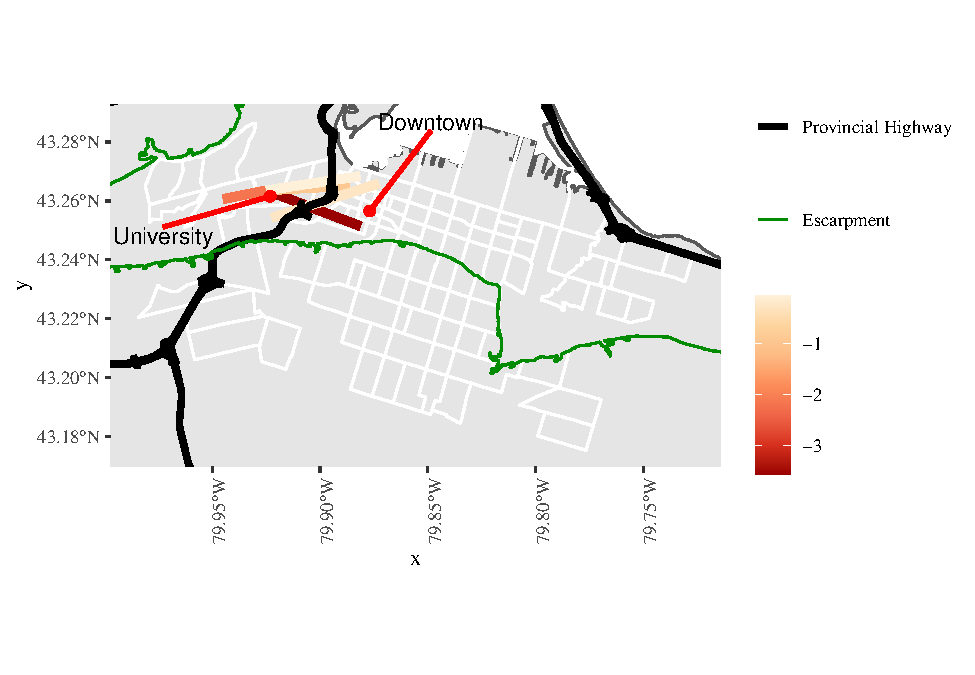
\includegraphics{Correlates-cycling-flows-routes_files/figure-latex/residuals-over-1.pdf}
\caption{\label{fig:residuals-overestimated} Map of Over-predicted
Bicycle Trip Flows (Black lines are provincial highways and green line
is the Niagara Escarpment)}
\end{figure}

Similarly, by plotting the positive residuals, after removing all
origin-destination pairs with zero trips, bicycle trip flows that were
under-estimated were visualized in Figure
\ref{fig:residuals-underestimated}. Given that the majority of trip
flows were under-estimated, we visualized trip flows in different maps
according to their characteristics. Figure \ref{fig:residuals-over-5km}
shows a map of trip flows over 5 km and Figure
\ref{fig:residuals-under-5km} shows trip flows under 5 km. One fifth of
under-estimated trip flows, approximately 21\%, had a \emph{quietest}
distance route between 5 and 25 kilometres. Trip distance is an
important determinant of cycling for transport (Heinen, van Wee, and
Maat 2010), which suggests that the distance between origin and
destination could be the reason that these flows were under-estimated.
Furthermore, approximately 17\% of under-estimated trip flows occurred
within the suburban neighbourhoods on the Niagara Escarpment. Fewer
cycling trips were expected in this area of the city because bicycle
trips are typically less likely in low density areas where there are
fewer destinations that can be reached in short distances, as was found
to be the case in the United States (Pucher and Buehler 2006). It is
also worth noting in this case that Hamilton's suburban areas have far
less cycling facilities compared to the lower city, which reinforces the
car-centric design of these neighbourhoods. Finally, there is a
noteworthy cluster of trip flows in the city's downtown core of 5 km or
less. Nielsen and Skov-Petersen (2018) note that built environment
attributes are effective at different spatial scales. They uncovered
positive effects of cycling infrastructure within 1 km of the home on
the probability of cycling, providing evidence that proximity to cycling
facilities can influence transport mode choices (Nielsen and
Skov-Petersen 2018). We hypothesize that this cluster was
under-estimated because cycling infrastructure has been built more
extensively in the downtown core and is likely normalizing travel by
bicycle in this area. The connectivity of such infrastructure between
zone of origin and zone of destination may not have been captured in the
inferred routes used as the cost function, leading to under-estimation.
Likewise, the downtown core features a higher density of destinations
within a 1-5 km distance that people could comfortably reach by bicycle,
compared to residential-only neighbourhoods.

Analyzing the residuals of trip flows can be a helpful practice for
transportation planners to evaluate how well the existing cycling
network meets the needs of bicyclists. This is particularly useful in
developing cycling cities, like Hamilton, where local geographic
analysis is needed to better inform future investments in infrastructure
to better support mobility. Transportation planners can use the
residuals to identify flows that are not well served by cycling
facilities and uncover gaps in the network.

\begin{figure}
\centering
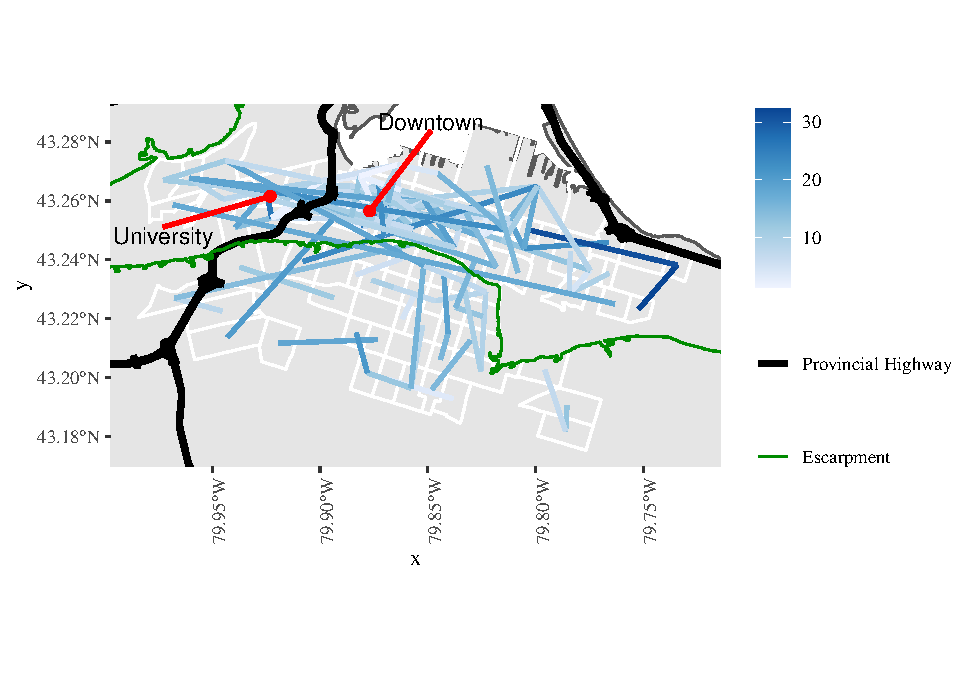
\includegraphics{Correlates-cycling-flows-routes_files/figure-latex/residuals-under-1.pdf}
\caption{\label{fig:residuals-underestimated} Map of Under-predicted
Bicycle Trip Flows (Black lines are provincial highways and green line
is the Niagara Escarpment)}
\end{figure}

\begin{figure}
\centering
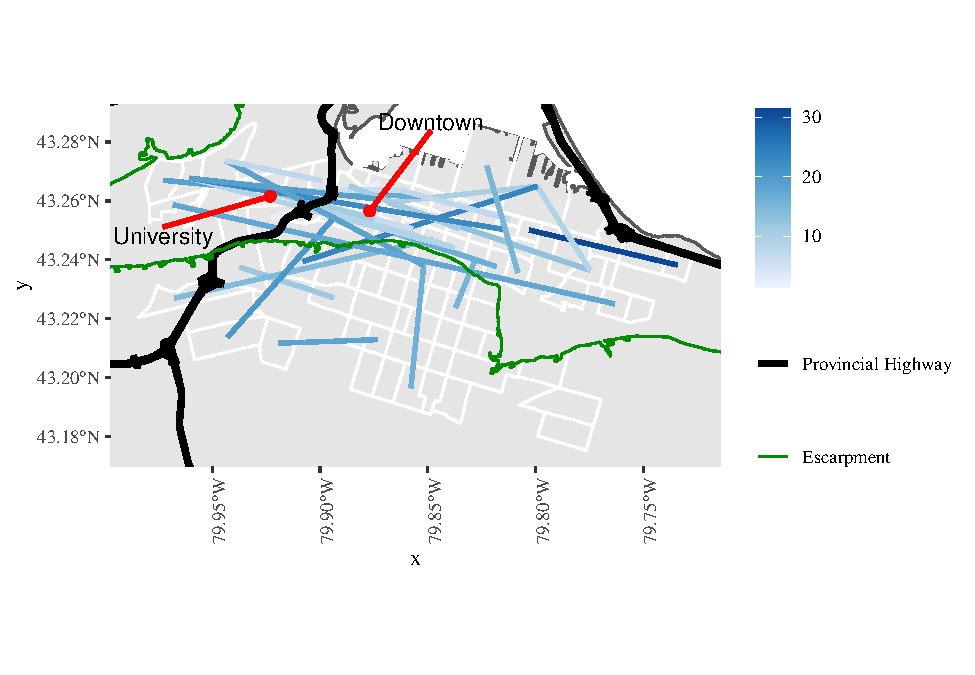
\includegraphics{Correlates-cycling-flows-routes_files/figure-latex/residuals-over-5km-1.pdf}
\caption{\label{fig:residuals-over-5km} Map of Under-predicted Bicycle
Trip Flows Over 5 km (Black lines are provincial highways and green line
is the Niagara Escarpment)}
\end{figure}

\begin{figure}
\centering
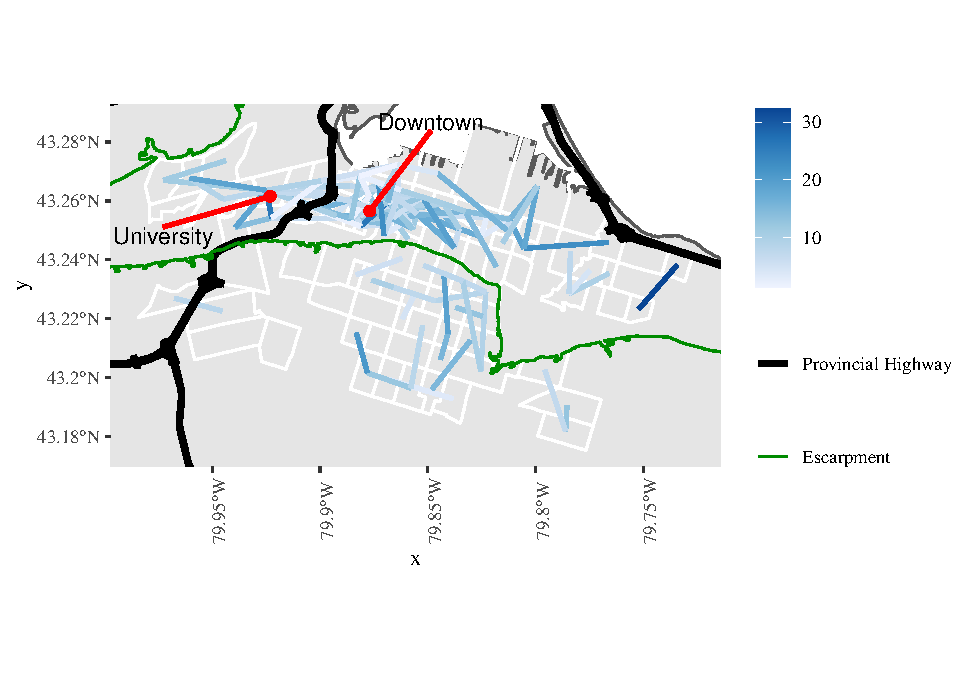
\includegraphics{Correlates-cycling-flows-routes_files/figure-latex/residuals-under-5km-1.pdf}
\caption{\label{fig:residuals-under-5km} Map of Under-predicted Bicycle
Trip Flows Less Than 5 km (Black lines are provincial highways and green
line is the Niagara Escarpment)}
\end{figure}

\hypertarget{limitations}{%
\subsection{Limitations}\label{limitations}}

Although there was no network autocorrelation in the final model, which
indicates that it sufficiently explains the observed pattern, the
findings may overemphasize the trip patterns of experienced cyclists.
Hamilton's cycling mode share is 1.2\% which means that it's highly
likely that bicyclists in the city at this time are ``strong and
fearless'' or ``enthused and confident'' riders (see Geller 2006). This
hypothesis is supported by the finding that approximately 21\% of
under-estimated trip flows were between 5 and 25 kilometres, which is
longer than the conventional bikeable distance. New or inexperienced
bicyclists would probably be uncomfortable travelling for such long
distances. The \emph{CycleStreets}
documentation\footnote{https://CRAN.R-project.org/package=cyclestreets}
acknowledges that routes inferred by the algorithm ``emulate the routes
taken by a knowledgeable cyclist''. This means that the inferred routes
used as a cost variable in our model may only be appealing to bicyclists
who are experienced and potentially more comfortable navigating a
developing cycling city with a fragmented cycle network. In this
respect, the \emph{quietest-distance} routes that best explained the
pattern of cycling flows in Hamilton may not represent routes that would
be considered ``quiet'' or safe enough by groups that are often
underrepresented in cycling such as women, children, and older adults.

\emph{CycleStreets} can infer a maximum of six routes that are rated
\emph{fastest}, \emph{quietest}, and \emph{balanced} using either
distance or time. While the \emph{quietest} distance routes best
explained the pattern of cycling trip flows, these are not the only
attractive or preferred routes between zones of origin and destination.
There are other routes or combinations of routes that incorporate
existing infrastructure which reflect individual tolerance mixing with
traffic or infrastructure preferences. Routes travelled by the ``strong
and fearless'' are not necessarily the same as routes travelled the
``interested but concerned''. Therefore, one of the limitations of using
an open source routing algorithm is that it does not currently consider
route preferences of bicyclists in Hamilton. However, it does give
streets with infrastructure a higher \emph{quietest} percentage score,
and we know from the literature that bicyclists prefer separated and
protected infrastructure (Buehler and Dill 2016). In another forthcoming
paper, we used photo elicitation to explore whether some of the inferred
routes were known to local bicyclists in Hamilton and confirmed that the
algorithm does select routes that are indeed commonly travelled
{[}Desjardins et al.~2020b submitted for publication{]}.

\hypertarget{sec:conclusion}{%
\section{Conclusion}\label{sec:conclusion}}

The objective of this study was to address the following questions: 1)
\emph{Which attributes at the zones of origin and destination influence
cycling trip flows in Hamilton?}; and 2) \emph{Which type of route best
explains the pattern of travel by bicycle in Hamilton?}. The use of a
spatial interaction model is methodologically more holistic than trip
generation analysis, an approach often used in the cycling literature
(for instance, see Noland, Smart, and Guo 2016), because it considered
attributes at the zones of origin and destination, as well as route
characteristics to estimate cyclist travel. Use of a routing algorithm
like \emph{CycleStreets} also constitutes a novel approach to overcome
the limitation of travel surveys. \emph{CycleStreets} enabled us to
experiment with different types of routes that knowledgeable and
experienced bicyclists may seek out. The model revealed that
shortest-distance \emph{quietest} routes that allow bicyclists to avoid
traffic best explain the pattern of cycling trip flows in Hamilton. In
addition, the availability of jobs and different land uses and
destinations at the end of the trip were positive attractors of bicycle
trips. Commercial locations and other destinations at the zone of
origin, as well as topography, had a negative influence on the number of
expected bicycle trips. Other important practical findings include that
the misspecification in the analysis of bicycle trip flows is evident in
the form of network autocorrelation - this has been known for other
types of flows, but as far as we know, has never been reported in the
cycling literature. By testing for network autocorrelation, we are
confident in the final model, which not only accounts for various
pull-push factors and cost measures, but also indicates that the model
sufficiently describes the pattern observed. Finally, analysis of the
model residuals to identify under- and over-estimated trip flows was
also suggestive in terms of other information about potential cycling
routes.

The approach adopted in this research also presents future opportunities
to systematically investigate the built environment along the inferred
routes. For instance, shortest-path \emph{quietest} routes may have
attributes that promote travel by bicycle, such as infrastructure or a
large proportion of residential streets, which leads to more cycling
than expected from the model. To test this assumption, environmental
audits were conducted along \emph{quietest} routes for a selection of
origin-destination pairs that were under-predicted in order to document
the presence or absence of features that may influence cycling (a
similar approach was employed in Moniruzzaman and Páez 2012). The
documentation of built environment attributes would contribute to our
understanding of what cyclists experience as they travel through a
developing cycling city like Hamilton, as well as validate whether the
inferred routes match where cyclists do indeed travel. This is the topic
of another forthcoming paper {[}Desjardins et al.~2020b submitted for
publication{]}.

\hypertarget{sec:acknowledgments}{%
\section{Acknowledgments}\label{sec:acknowledgments}}

The authors wish to express their gratitude to Yongwan Chun and Roberto
Patuelli for sharing their \texttt{R} code for the Jacqmin-Gadda's \(T\)
test. The authors would also like to thank the three anonymous reviewers
for their constructive feedback. In addition, the following \texttt{R}
packages were used in the course of this investigation and the authors
wish to acknowledge their developers: \texttt{cyclestreets} (Lovelace
and Lucas-Smith 2018), \texttt{ggthemes} (Arnold 2019),
\texttt{kableExtra} (Zhu 2019), \texttt{knitr}(Xie 2014, 2015),
\texttt{rticles} (Allaire et al. 2020), \texttt{sf} (Pebesma 2018),
\texttt{spdep} (Bivand, Pebesma, and Gomez-Rubio 2013),
\texttt{tidyverse} (Wickham et al. 2019), \texttt{units} (Pebesma,
Mailund, and Hiebert 2016), and \texttt{zeligverse} (Gandrud 2017).

\hypertarget{references}{%
\section*{References}\label{references}}
\addcontentsline{toc}{section}{References}

\hypertarget{refs}{}
\leavevmode\hypertarget{ref-Adam2020}{}%
Adam, Lukas, Tim Jones, and Marco te Brömmelstroet. 2020. ``Planning for
Cycling in the Dispersed City: Establishing a Hierarchy of Effectiveness
of Municipal Cycling Policies.'' \emph{Transportation} 47 (2): 503--27.
\url{https://doi.org/10.1007/s11116-018-9878-3}.

\leavevmode\hypertarget{ref-Allaire2020}{}%
Allaire, JJ, Yihui Xie, R Foundation, Hadley Wickham, Journal of
Statistical Software, Ramnath Vaidyanathan, Association for Computing
Machinery, et al. 2020. \emph{Rticles: Article Formats for R Markdown}.
Manual.

\leavevmode\hypertarget{ref-Arnold2019}{}%
Arnold, Jeffrey B. 2019. \emph{Ggthemes: Extra Themes, Scales and Geoms
for 'Ggplot2'}. Manual.

\leavevmode\hypertarget{ref-Assuncao2019}{}%
Assunçao-Denis, Marie-Ève, and Ray Tomalty. 2019. ``Increasing Cycling
for Transportation in Canadian Communities: Understanding What Works.''
\emph{Transportation Research Part A: Policy and Practice} 123 (May):
288--304. \url{https://doi.org/10.1016/j.tra.2018.11.010}.

\leavevmode\hypertarget{ref-Avila2018}{}%
Avila-Palencia, I, L Int Panis, E Dons, and M et al. Gaupp-Berghausen.
2018. ``The Effects of Transport Mode Use on Self-Perceived Health,
Mental Health, and Social Contact Measures: A Cross-Sectional and
Longitudinal Study.'' Journal Article. \emph{Environment International}
120: 199--206. \url{https://doi.org/10.1016/j.envint.2018.08.002}.

\leavevmode\hypertarget{ref-Bivand2013}{}%
Bivand, Roger S., Edzer Pebesma, and Virgilio Gomez-Rubio. 2013.
\emph{Applied Spatial Data Analysis with R, Second Edition}. Springer,
NY.

\leavevmode\hypertarget{ref-Branion2019}{}%
Branion-Calles, Michael, Trisalyn Nelson, Daniel Fuller, Lise Gauvin,
and Meghan Winters. 2019. ``Associations Between Individual
Characteristics, Availability of Bicycle Infrastructure, and City-Wide
Safety Perceptions of Bicycling: A Cross-Sectional Survey of Bicyclists
in 6 Canadian and U.S. Cities.'' \emph{Transportation Research Part A:
Policy and Practice} 123 (May): 229--39.
\url{https://doi.org/10.1016/j.tra.2018.10.024}.

\leavevmode\hypertarget{ref-Broach2012}{}%
Broach, Joseph, Jennifer Dill, and John Gliebe. 2012. ``Where Do
Cyclists Ride? A Route Choice Model Developed with Revealed Preference
GPS Data.'' \emph{Transportation Research Part A: Policy and Practice}
46 (10): 1730--40. \url{https://doi.org/10.1016/j.tra.2012.07.005}.

\leavevmode\hypertarget{ref-brunsdon2020opening}{}%
Brunsdon, Chris, and Alexis Comber. 2020. ``Opening Practice: Supporting
Reproducibility and Critical Spatial Data Science.'' \emph{Journal of
Geographical Systems}, 1--20.
\url{https://doi.org/10.1007/s10109-020-00334-2}.

\leavevmode\hypertarget{ref-Buehler2016}{}%
Buehler, Ralph, and Jennifer Dill. 2016. ``Bikeway Networks: A Review of
Effects on Cycling.'' \emph{Transport Reviews} 36 (1): 9--27.
\url{https://doi.org/10.1080/01441647.2015.1069908}.

\leavevmode\hypertarget{ref-Buehler2012}{}%
Buehler, Ralph, and John Pucher. 2012. ``Cycling to Work in 90 Large
American Cities: New Evidence on the Role of Bike Paths and Lanes.''
\emph{Transportation} 39 (2): 409--32.
\url{https://doi.org/10.1007/s11116-011-9355-8}.

\leavevmode\hypertarget{ref-Celis2017}{}%
Celis-Morales, CA, DM Lyall, and P et al. Welsh. 2017. ``Association
Between Active Commuting and Incident Cardiovascular Disease, Cancer,
and Mortality: Prospective Cohort Study.'' Journal Article. \emph{BMJ
(Clinical Research Ed.)} 357: j1456.
\url{https://doi.org/10.1136/bmj.j1456}.

\leavevmode\hypertarget{ref-Cervero2019}{}%
Cervero, Robert, Steve Denman, and Ying Jin. 2019. ``Network Design,
Built and Natural Environments, and Bicycle Commuting: Evidence from
British Cities and Towns.'' \emph{Transport Policy} 74 (February):
153--64. \url{https://doi.org/10.1016/j.tranpol.2018.09.007}.

\leavevmode\hypertarget{ref-Chen2018}{}%
Chen, Peng, Qing Shen, and Suzanne Childress. 2018. ``A GPS Data-Based
Analysis of Built Environment Influences on Bicyclist Route
Preferences.'' \emph{International Journal of Sustainable
Transportation} 12 (3): 218--31.
\url{https://doi.org/10.1080/15568318.2017.1349222}.

\leavevmode\hypertarget{ref-Chun2008}{}%
Chun, Yongwan. 2008. ``Modeling Network Autocorrelation Within Migration
Flows by Eigenvector Spatial Filtering.'' \emph{Journal of Geographical
Systems} 10 (4): 317--44.
\url{https://doi.org/10.1007/s10109-008-0068-2}.

\leavevmode\hypertarget{ref-Calgary2011}{}%
City of Calgary. 2011. ``Cycling Strategy.''
https://www.calgary.ca/Transportation/TP/Documents/cycling/Cycling-Strategy/2011-cycling-strategy-presentation.pdf.

\leavevmode\hypertarget{ref-Tmp2018}{}%
City of Hamilton. 2018a. ``City of Hamilton Transportation Master Plan
Review and Update.''
https://www.hamilton.ca/sites/default/files/media/browser/2018-10-24/tmp-review-update-final-report-oct2018.pdf.

\leavevmode\hypertarget{ref-Cmp2018}{}%
---------. 2018b. ``Cycling Master Plan Review and Update.''
https://www.hamilton.ca/sites/default/files/media/browser/2018-06-06/draft-tmp-backgroundreport-cyclingmp-11-1.pdf.

\leavevmode\hypertarget{ref-Cmp2009}{}%
---------. 2018c. ``Shifting Gears 2009: Hamilton's Cycling Master Plan
Review and Update.''
https://www.hamilton.ca/sites/default/files/media/browser/2014-12-17/cycling-master-plan-chapters-1-2-3.pdf.

\leavevmode\hypertarget{ref-Montreal2017}{}%
City of Montreal. 2017. ``Montreal, City of Cyclists; Cycling Master
Plan: Safety, Efficiency, Audacity.''
https://ville.montreal.qc.ca/pls/portal/docs/page/transports\_fr/media/documents/plan\_cadre\_velo\_ang\_final\_lr.pdf.

\leavevmode\hypertarget{ref-Vancouver2012}{}%
City of Vancouver. 2012. ``Transportation 2040: Moving Forward.''
https://vancouver.ca/files/cov/transportation-2040-plan.pdf.

\leavevmode\hypertarget{ref-ColeHunter2015}{}%
Cole-Hunter, T, D Donaire-Gonzalez, A Curto, A Ambros, A Valentin, J
Garcia-Aymerich, D Martínez, et al. 2015. ``Objective Correlates and
Determinants of Bicycle Commuting Propensity in an Urban Environment.''
\emph{Transportation Research Part D: Transport and Environment} 40
(October): 132--43. \url{https://doi.org/10.1016/j.trd.2015.07.004}.

\leavevmode\hypertarget{ref-Dmg2014tts}{}%
Data Management Group. 2014. ``2011 TTS: Design and Conduct of the
Survey.'' http://dmg.utoronto.ca/pdf/tts/2011/conduct2011.pdf.

\leavevmode\hypertarget{ref-Dmg2018tts}{}%
---------. 2018. ``2016 TTS: Design and Conduct of the Survey.''
http://dmg.utoronto.ca/pdf/tts/2016/2016TTS\_Conduct.pdf.

\leavevmode\hypertarget{ref-deNazelle2011}{}%
De Nazelle, Audrey, Mark J Nieuwenhuijsen, Josep M Antó, Michael Brauer,
David Briggs, Charlotte Braun-Fahrlander, Nick Cavill, et al. 2011.
``Improving Health Through Policies That Promote Active Travel: A Review
of Evidence to Support Integrated Health Impact Assessment.''
\emph{Environment International} 37 (4): 766--77.

\leavevmode\hypertarget{ref-Dill2003}{}%
Dill, J, and T Carr. 2003. ``Bicycle Commuting and Facilities in Major
U.S. Cities: If You Build Them, Commuters Will Use Them.'' Journal
Article. \emph{Transportation Research Record: Journal of the
Transportation Research Board} 1828.

\leavevmode\hypertarget{ref-Dill2009}{}%
Dill, Jennifer. 2009. ``Bicycling for Transportation and Health: The
Role of Infrastructure.'' \emph{Journal of Public Health Policy} 30
(S1): S95--S110. \url{https://doi.org/10.1057/jphp.2008.56}.

\leavevmode\hypertarget{ref-deDios2011Modelling}{}%
Dios Ortúzar, Juan de, and Luis G Willumsen. 2011. \emph{Modelling
Transport}. Fourth. John wiley \& sons.

\leavevmode\hypertarget{ref-elAssi2017effects}{}%
El-Assi, Wafic, Mohamed Salah Mahmoud, and Khandker Nurul Habib. 2017.
``Effects of Built Environment and Weather on Bike Sharing Demand: A
Station Level Analysis of Commercial Bike Sharing in Toronto.''
\emph{Transportation} 44 (3): 589--613.

\leavevmode\hypertarget{ref-Gandrud2017}{}%
Gandrud, Christopher. 2017. \emph{Zeligverse: Easily Install and Load
Stable Zelig Packages}. Manual.

\leavevmode\hypertarget{ref-Geller2006}{}%
Geller, Roger. 2006. ``Four Types of Cyclists.''
https://www.portlandoregon.gov/transportation/44597?a=237507.

\leavevmode\hypertarget{ref-Griffith2011}{}%
Griffith, Daniel A. 2011. ``Visualizing Analytical Spatial
Autocorrelation Components Latent in Spatial Interaction Data: An
Eigenvector Spatial Filter Approach.'' \emph{Computers, Environment and
Urban Systems} 35 (2): 140--49.
\url{https://doi.org/10.1016/j.compenvurbsys.2010.08.003}.

\leavevmode\hypertarget{ref-griffithConstrainedVariantsGravity2016}{}%
Griffith, Daniel A., and Manfred M. Fischer. 2016. ``Constrained
Variants of the Gravity Model and Spatial Dependence: Model
Specification and Estimation Issues.'' In \emph{Spatial Econometric
Interaction Modelling}, edited by Roberto Patuelli and Giuseppe Arbia,
37--66. Advances in Spatial Science. Cham: Springer International
Publishing. \url{https://doi.org/10.1007/978-3-319-30196-9_3}.

\leavevmode\hypertarget{ref-Hamilton2019}{}%
Hamilton, City of. n.d. ``Mountain Climber Pilot Program Expanded.''
https://www.hamilton.ca/government-information/news-centre/news-releases/mountain-climber-pilot-program-expanded.

\leavevmode\hypertarget{ref-handyMakingUSCities2020}{}%
Handy, Susan. 2020. ``Making US Cities Pedestrian- and
Bicycle-Friendly.'' In \emph{Transportation, Land Use, and Environmental
Planning}, edited by Elizabeth Deakin, 169--87. Elsevier.
\url{https://doi.org/10.1016/B978-0-12-815167-9.00009-8}.

\leavevmode\hypertarget{ref-handyPromotingCyclingTransport2014}{}%
Handy, Susan, Bert van Wee, and Maarten Kroesen. 2014. ``Promoting
Cycling for Transport: Research Needs and Challenges.'' \emph{Transport
Reviews} 34: 4--24.

\leavevmode\hypertarget{ref-Heesch2015}{}%
Heesch, Kristiann C., Billie Giles-Corti, and Gavin Turrell. 2015.
``Cycling for Transport and Recreation: Associations with the
Socio-Economic, Natural and Built Environment.'' \emph{Health \& Place}
36 (November): 152--61.
\url{https://doi.org/10.1016/j.healthplace.2015.10.004}.

\leavevmode\hypertarget{ref-heinenCommutingBicycleOverview2010}{}%
Heinen, Eva, Bert van Wee, and Kees Maat. 2010. ``Commuting by Bicycle:
An Overview of the Literature.'' \emph{Transport Reviews} 30: 59--96.

\leavevmode\hypertarget{ref-Jacqmin1997}{}%
Jacqmin-Gadda, Hélène, Daniel Commenges, Chakib Nejjari, and
Jean-François Dartigues. 1997. ``Tests of Geographical Correlation with
Adjustment for Explanatory Variables: An Application to Dyspnoea in the
Elderly.'' \emph{Statistics in Medicine} 16 (11): 1283--97.

\leavevmode\hypertarget{ref-Le2018}{}%
Le, Huyen T. K., Ralph Buehler, and Steve Hankey. 2018. ``Correlates of
the Built Environment and Active Travel: Evidence from 20 US
Metropolitan Areas.'' \emph{Environmental Health Perspectives} 126 (7):
077011. \url{https://doi.org/10.1289/EHP3389}.

\leavevmode\hypertarget{ref-liuWhatMakesGood2020}{}%
Liu, George, Samuel Nello-Deakin, Marco Brommelstroet te, and Yuki
Yamamoto. 2020. ``What Makes a Good Cargo Bike Route? Perspectives from
Users and Planners.'' \emph{American Journal of Economics and Sociology}
73: 941--65. \url{https://doi.org/10.1111/ajes.12332}.

\leavevmode\hypertarget{ref-lovelaceOpenSourceTools2021}{}%
Lovelace, Robin. 2021. ``Open Source Tools for Geographic Analysis in
Transport Planning.'' \emph{Journal of Geographical Systems}, January.
\url{https://doi.org/10.1007/s10109-020-00342-2}.

\leavevmode\hypertarget{ref-Lovelace2018}{}%
Lovelace, Robin, and Martin Lucas-Smith. 2018. \emph{Cyclestreets: Cycle
Routing and Data for Cycling Advocacy}. Manual.

\leavevmode\hypertarget{ref-Lu2018understanding}{}%
Lu, Wei, Darren M Scott, and Ron Dalumpines. 2018. ``Understanding Bike
Share Cyclist Route Choice Using GPS Data: Comparing Dominant Routes and
Shortest Paths.'' \emph{Journal of Transport Geography} 71: 172--81.

\leavevmode\hypertarget{ref-McArthur2019}{}%
McArthur, David Philip, and Jinhyun Hong. 2019. ``Visualising Where
Commuting Cyclists Travel Using Crowdsourced Data.'' \emph{Journal of
Transport Geography} 74 (January): 233--41.
\url{https://doi.org/10.1016/j.jtrangeo.2018.11.018}.

\leavevmode\hypertarget{ref-Mertens2017}{}%
Mertens, Lieze, Sofie Compernolle, Benedicte Deforche, Joreintje D.
Mackenbach, Jeroen Lakerveld, Johannes Brug, Célina Roda, et al. 2017.
``Built Environmental Correlates of Cycling for Transport Across
Europe.'' \emph{Health \& Place} 44 (March): 35--42.
\url{https://doi.org/10.1016/j.healthplace.2017.01.007}.

\leavevmode\hypertarget{ref-Metulini2018}{}%
Metulini, Rodolfo, Roberto Patuelli, and Daniel Griffith. 2018. ``A
Spatial-Filtering Zero-Inflated Approach to the Estimation of the
Gravity Model of Trade.'' \emph{Econometrics} 6 (1): 9.
\url{https://doi.org/10.3390/econometrics6010009}.

\leavevmode\hypertarget{ref-Mitra2016}{}%
Mitra, R, N Smith Lea, I Cantello, and G Hanson. 2016. ``Cycling
Behaviour and Potential in the Greater Toronto and Hamilton Area.''
http://transformlab.ryerson.ca/wp-content/uploads/2016/10/Cycling-potential-in-GTHA-final-report-2016.pdf.

\leavevmode\hypertarget{ref-Moniruzzaman2012}{}%
Moniruzzaman, M.d., and A Páez. 2012. ``A Model-Based Approach to Select
Case Sites for Walkability Audits.'' Journal Article. \emph{Health \&
Place} 18 (6): 1323--34.
\url{https://doi.org/10.1016/j.healthplace.2012.09.013}.

\leavevmode\hypertarget{ref-Moniruzzaman2016}{}%
---------. 2016. ``An Investigation of the Attributes of Walkable
Environments from the Perspective of Seniors in Montreal.'' Journal
Article. \emph{Journal of Transport Geography} 51: 85--96.
\url{https://doi.org/http://dx.doi.org/10.1016/j.jtrangeo.2015.12.001}.

\leavevmode\hypertarget{ref-Moudon2003walking}{}%
Moudon, Anne Vernez, and Chanam Lee. 2003. ``Walking and Bicycling: An
Evaluation of Environmental Audit Instruments.'' \emph{American Journal
of Health Promotion} 18 (1): 21--37.

\leavevmode\hypertarget{ref-moudonCyclingBuiltEnvironment2005a}{}%
Moudon, Anne Vernez, Chanam Lee, Allen D. Cheadle, Cheza W. Collier,
Donna Johnson, Thomas L. Schmid, and Robert D. Weather. 2005. ``Cycling
and the Built Environment, a US Perspective.'' \emph{Transportation
Research Part D: Transport and Environment} 10 (3): 245--61.

\leavevmode\hypertarget{ref-Nielsen2018}{}%
Nielsen, Thomas Alexander Sick, and Hans Skov-Petersen. 2018.
``Bikeability Urban Structures Supporting Cycling. Effects of Local,
Urban and Regional Scale Urban Form Factors on Cycling from Home and
Workplace Locations in Denmark.'' \emph{Journal of Transport Geography}
69 (May): 36--44. \url{https://doi.org/10.1016/j.jtrangeo.2018.04.015}.

\leavevmode\hypertarget{ref-nolandBikeshareTripGeneration2016}{}%
Noland, Robert B., Michael J. Smart, and Ziye Guo. 2016. ``Bikeshare
Trip Generation in New York City.'' \emph{Transportation Research Part
A: Policy and Practice} 94: 164--81.
\url{https://doi.org/10.1016/j.tra.2016.08.030}.

\leavevmode\hypertarget{ref-Nordengen2019}{}%
Nordengen, Ruther, Riiser, Andersen, and Solbraa. 2019. ``Correlates of
Commuter Cycling in Three Norwegian Counties.'' \emph{International
Journal of Environmental Research and Public Health} 16 (22): 4372.
\url{https://doi.org/10.3390/ijerph16224372}.

\leavevmode\hypertarget{ref-Oja2011}{}%
Oja, P., S. Titze, A. Bauman, B. de Geus, P. Krenn, B. Reger-Nash, and
T. Kohlberger. 2011. ``Health Benefits of Cycling: A Systematic
Review.'' \emph{Scandinavian Journal of Medicine \& Science in Sports}
21 (4): 496--509.
\url{https://doi.org/10.1111/j.1600-0838.2011.01299.x}.

\leavevmode\hypertarget{ref-paezEnjoymentCommuteComparison2010}{}%
Páez, Antonio, and Kate Whalen. 2010. ``Enjoyment of Commute: A
Comparison of Different Transportation Modes.'' \emph{Transportation
Research Part A: Policy and Practice} 44 (7): 537--49.
\url{https://doi.org/10.1016/j.tra.2010.04.003}.

\leavevmode\hypertarget{ref-Pebesma2018}{}%
Pebesma, Edzer. 2018. ``Simple Features for R: Standardized Support for
Spatial Vector Data.'' \emph{The R Journal} 10 (1): 439--46.
\url{https://doi.org/10.32614/RJ-2018-009}.

\leavevmode\hypertarget{ref-Pebesma2016}{}%
Pebesma, Edzer, Thomas Mailund, and James Hiebert. 2016. ``Measurement
Units in R.'' \emph{R Journal} 8 (2): 486--94.
\url{https://doi.org/10.32614/RJ-2016-061}.

\leavevmode\hypertarget{ref-Pritchard2018}{}%
Pritchard, Ray. 2018. ``Revealed Preference Methods for Studying Bicycle
Route Choice - a Systematic Review.'' \emph{International Journal of
Environmental Research and Public Health} 15 (3): 470.
\url{https://doi.org/10.3390/ijerph15030470}.

\leavevmode\hypertarget{ref-Pritchard2019}{}%
Pritchard, Ray, Dominik Bucher, and Yngve Frøyen. 2019. ``Does New
Bicycle Infrastructure Result in New or Rerouted Bicyclists? A
Longitudinal GPS Study in Oslo.'' \emph{Journal of Transport Geography}
77 (May): 113--25. \url{https://doi.org/10.1016/j.jtrangeo.2019.05.005}.

\leavevmode\hypertarget{ref-Pucher2006}{}%
Pucher, John, and Ralph Buehler. 2006. ``Why Canadians Cycle More Than
Americans: A Comparative Analysis of Bicycling Trends and Policies.''
\emph{Transport Policy} 13 (3): 265--79.
\url{https://doi.org/10.1016/j.tranpol.2005.11.001}.

\leavevmode\hypertarget{ref-Rodrigue2020}{}%
Rodrigue, Jean-Paul. 2020. \emph{The Geography of Transport Systems}.
Fifth. Routledge.

\leavevmode\hypertarget{ref-Sallis2013}{}%
Sallis, James F., Terry L. Conway, Lianne I. Dillon, Lawrence D. Frank,
Marc A. Adams, Kelli L. Cain, and Brian E. Saelens. 2013.
``Environmental and Demographic Correlates of Bicycling.''
\emph{Preventive Medicine} 57 (5): 456--60.
\url{https://doi.org/10.1016/j.ypmed.2013.06.014}.

\leavevmode\hypertarget{ref-Sarjala2019}{}%
Sarjala, Satu. 2019. ``Built Environment Determinants of Pedestrians'
and Bicyclists' Route Choices on Commute Trips: Applying a New
Grid-Based Method for Measuring the Built Environment Along the Route.''
\emph{Journal of Transport Geography} 78 (June): 56--69.
\url{https://doi.org/10.1016/j.jtrangeo.2019.05.004}.

\leavevmode\hypertarget{ref-Schneider2015}{}%
Schneider, Robert J., and Joseph Stefanich. 2015. ``Neighborhood
Characteristics That Support Bicycle Commuting: Analysis of the Top 100
U.S. Census Tracts.'' \emph{Transportation Research Record: Journal of
the Transportation Research Board} 2520: 41--51.
\url{https://doi.org/DOI:\%2010.3141/2520-06}.

\leavevmode\hypertarget{ref-Scott2019factors}{}%
Scott, Darren M, and Celenna Ciuro. 2019. ``What Factors Influence Bike
Share Ridership? An Investigation of Hamilton, Ontario's Bike Share
Hubs.'' \emph{Travel Behaviour and Society} 16: 50--58.

\leavevmode\hypertarget{ref-scottRouteChoiceBike2021}{}%
Scott, Darren M., Wei Lu, and Matthew J. Brown. 2021. ``Route Choice of
Bike Share Users: Leveraging GPS Data to Derive Choice Sets.''
\emph{Journal of Transport Geography} 90 (January): 102903.
\url{https://doi.org/10.1016/j.jtrangeo.2020.102903}.

\leavevmode\hypertarget{ref-SkovPetersen2018}{}%
Skov-Petersen, Hans, Bernhard Barkow, Thomas Lundhede, and Jette Bredahl
Jacobsen. 2018. ``How Do Cyclists Make Their Way? - A GPS-Based Revealed
Preference Study in Copenhagen.'' \emph{International Journal of
Geographical Information Science} 32 (7): 1469--84.
\url{https://doi.org/10.1080/13658816.2018.1436713}.

\leavevmode\hypertarget{ref-solisOpenGeospatialTools2020}{}%
Solís, Patricia, Jennings Anderson, and Sushil Rajagopalan. 2020. ``Open
Geospatial Tools for Humanitarian Data Creation, Analysis, and Learning
Through the Global Lens of YouthMappers.'' \emph{Journal of Geographical
Systems}, November. \url{https://doi.org/10.1007/s10109-020-00339-x}.

\leavevmode\hypertarget{ref-Statscan2017}{}%
Statistics Canada. 2017. ``Journey to Work: Key Results from the 2016
Census.''
https://www150.statcan.gc.ca/n1/en/daily-quotidien/171129/dq171129c-eng.pdf?st=eVPg5Nih.

\leavevmode\hypertarget{ref-Verlinden2019}{}%
Verlinden, Y and Manaugh, K and Savan, B and Smith Lea, N and Tomalty, R
and Winters, M. 2019. ``Increasing Cycling in Canada: A Guide to What
Works.''
https://www.tcat.ca/wp-content/uploads/2019/09/Increasing-Cycling-in-Canada-A-Guide-to-What-Works-2019-09-25.pdf.

\leavevmode\hypertarget{ref-Wickham2019}{}%
Wickham, Hadley, Mara Averick, Jennifer Bryan, Winston Chang, Lucy
D'Agostino McGowan, Romain François, Garrett Grolemund, et al. 2019.
``Welcome to the tidyverse.'' \emph{Journal of Open Source Software} 4
(43): 1686. \url{https://doi.org/10.21105/joss.01686}.

\leavevmode\hypertarget{ref-Winters2010}{}%
Winters, Meghan, Michael Brauer, Eleanor M. Setton, and Kay Teschke.
2010. ``Built Environment Influences on Healthy Transportation Choices:
Bicycling Versus Driving.'' \emph{Journal of Urban Health} 87 (6):
969--93. \url{https://doi.org/10.1007/s11524-010-9509-6}.

\leavevmode\hypertarget{ref-Xie2014}{}%
Xie, Yihui. 2014. ``Knitr: A Comprehensive Tool for Reproducible
Research in R.'' In \emph{Implementing Reproducible Computational
Research}, edited by Victoria Stodden, Friedrich Leisch, and Roger D.
Peng. Chapman and Hall/CRC.

\leavevmode\hypertarget{ref-Xie2015}{}%
---------. 2015. \emph{Dynamic Documents with R and Knitr}. Second. Boca
Raton, Florida: Chapman and Hall/CRC.

\leavevmode\hypertarget{ref-yangCyclingfriendlyCityUpdated2019}{}%
Yang, Yiyang, Xueying Wu, Peiling Zhao, Zhonghua Gou, and Yi Lu. 2019.
``Towards a Cycling-Friendly City: An Updated Review of the Associations
Between Built Environment and Cycling Behaviors (20072017).''
\emph{Journal of Transport \& Health} 14: 100613.
\url{https://doi.org/10.1016/j.jth.2019.100613}.

\leavevmode\hypertarget{ref-Zahabi2016}{}%
Zahabi, Seyed Amir H., Annie Chang, Luis F. Miranda-Moreno, and Zachary
Patterson. 2016. ``Exploring the Link Between the Neighborhood
Typologies, Bicycle Infrastructure and Commuting Cycling over Time and
the Potential Impact on Commuter GHG Emissions.'' \emph{Transportation
Research Part D: Transport and Environment} 47 (August): 89--103.
\url{https://doi.org/10.1016/j.trd.2016.05.008}.

\leavevmode\hypertarget{ref-Zhao2014}{}%
Zhao, Pengjun. 2014. ``The Impact of the Built Environment on Bicycle
Commuting: Evidence from Beijing.'' \emph{Urban Studies} 51 (5):
1019--37. \url{https://doi.org/10.1177/0042098013494423}.

\leavevmode\hypertarget{ref-Zhu2019}{}%
Zhu, Hao. 2019. \emph{kableExtra: Construct Complex Table with 'Kable'
and Pipe Syntax}. Manual.


\bibliographystyle{spphys}
\bibliography{References.bib}

\end{document}
